\documentclass{report}
\usepackage[utf8]{inputenc}
%use british to avoid words separating randomly at the end of lines:
\usepackage[british]{babel}

\usepackage[toc,page]{appendix}

%plots
\usepackage{pgfplots}
\pgfplotsset{width=8cm,compat=1.9}
%reducing graph compilation time
\usepgfplotslibrary{external}
\tikzexternalize

%multi-line comments
\usepackage{comment}

%simboli matematici in più
\usepackage{amsmath}
\usepackage{amssymb}
\usepackage{dsfont}
\usepackage{mathtools}
\usepackage{mathrsfs}

% bold greek symbols
\usepackage{bm}

%code listing:
\usepackage{listings}
%listing style:
\definecolor{codegreen}{rgb}{0,0.6,0}
\definecolor{codegray}{rgb}{0.5,0.5,0.5}
\definecolor{codepurple}{rgb}{0.58,0,0.82}
\definecolor{backcolour}{rgb}{0.95,0.95,0.92}

\lstdefinestyle{mystyle}{
    backgroundcolor=\color{backcolour},   
    commentstyle=\color{codegreen},
    keywordstyle=\color{magenta},
    numberstyle=\tiny\color{codegray},
    stringstyle=\color{codepurple},
    basicstyle=\ttfamily\footnotesize,
    breakatwhitespace=false,         
    breaklines=true,                 
    captionpos=b,                    
    keepspaces=true,                 
    numbers=left,                    
    numbersep=5pt,                  
    showspaces=false,                
    showstringspaces=false,
    showtabs=false,                  
    tabsize=2
}
\lstset{style=mystyle,
moredelim=**[is][\color{blue} ]{@}{@}
}

%indexing theorems
\usepackage{amsthm}
%bold names for theorems 
\makeatletter
\def\th@plain{%
  \thm@notefont{}% same as heading font
  \itshape % body font
}
\def\th@definition{%
  \thm@notefont{}% same as heading font
  \normalfont % body font
}
\makeatother
\newtheorem{theorem}{Theorem}[section]
\newtheorem{corollary}{Corollary}[theorem]
\newtheorem{lemma}[theorem]{Lemma}
\newtheorem{definition}{Definition}[section]
\newtheorem{prop}{Proposition}[section]
\newtheorem{remark}[section]{Remark}

%references
\usepackage{hyperref}
\usepackage{cleveref}
\crefformat{section}{\S#2#1#3}
\crefformat{subsection}{\S#2#1#3}
\crefformat{subsubsection}{\S#2#1#3}
\crefrangeformat{section}{\S\S#3#1#4 to~#5#2#6}
\crefmultiformat{section}{\S\S#2#1#3}{ and~#2#1#3}{, #2#1#3}{ and~#2#1#3}

%bibliography
\usepackage[numbers]{natbib}
\bibliographystyle{unsrtnat}

%captions, figure and colors
\usepackage{graphicx}
\graphicspath{ {./img/}}
\usepackage[export]{adjustbox}
\usepackage[font=small,labelfont=bf, tableposition=top]{caption}
\usepackage[font=small]{subcaption}

%defining new commands
\newcommand{\Ex}{\`E\:}
\newcommand{\One}{\mathds{1}}
\newcommand{\rb}{\mathbb{R}}
\newcommand{\nb}{\mathbb{N}}
\newcommand{\zb}{\mathbb{Z}}
\newcommand{\Id}{\mathds{I}}
\newcommand{\de}{\partial}
\newcommand{\man}{\mathcal{M}}
\newcommand{\alp}{\mathcal{A}}
\newcommand{\ent}{\mathcal{S}}

%geometry of pages
\usepackage{geometry}
\usepackage{float}
\usepackage{titlesec}

\geometry{
	paper=a4paper, 
	inner=2.5cm, % Inner margin
	outer=3cm, % Outer margin
	bindingoffset=0.5cm, % Binding offset
	top=2.5cm, % Top margin
	bottom=3cm, % Bottom margin
	%showframe, % Uncomment to show how the type block is set on the page
}

\title{\textbf{Entropic Information Theory}}

\author{Matteo Falcioni \\ \url{https://github.com/Grufoony/Physics_Unibo}}
\date{}
\begin{document}

\maketitle
%eq. numerate per sezioni (3.1, 3.2...)
\numberwithin{equation}{section} 

%numbering pages + table of contents
\setcounter{page}{1}
\pagenumbering{arabic}
\tableofcontents{}

\chapter{Preliminaries}

\section{Ergodic Information Theory}
Information theory answers two fundamental questions in communication
theory: What is the ultimate data compression (answer: the entropy $H$),
and what is the ultimate transmission rate of communication (answer: the
channel capacity\footnote{Outside of the scope of this course} $C$ ). For this reason some consider information theory
to be a subset of communication theory. It can be argued that it is much more.
Indeed, it has fundamental contributions to make in statistical physics
(thermodynamics), computer science (Kolmogorov complexity or algorithmic complexity), statistical inference (Occam’s Razor: “The simplest
explanation is best”), and to probability and statistics (error exponents for
optimal hypothesis testing and estimation).
\\Information
theory intersects physics (statistical mechanics), mathematics (probability
theory), electrical engineering (communication theory), and computer science (algorithmic complexity). 

What about ergodicity? The world \textit{ergodic} was introduced by L. Boltzmann in the context of classical (statistical) mechanics to describe the action of the dynamics $T_t, \, t \in \rb$ over an energy surface $\Sigma_E$. Boltzmann had hoped that each orbit $\big\{ T_t, \, t \in \rb \big\}$ would equal the whole energy surface $\Sigma_E$ : he called this statement the \textit{ergodic hypothesis}. The word ergodic comes from the union of the greek words ergon (work) and odos (path). Boltzmann had in fact assumed this hypothesis in order to deduce the equality of time mean and space mean over the phase space, which is a fundamental algorithm in statistical mechanics. 
\\\textit{The ergodic hypothesis, as stated above, is \textbf{false}.} The property that phase flows need to satisfy in order for time and space means of real-valued function is now called \textit{ergodicity}.
\\Usually the term ergodic theory is used to refer to the study of the actions of groups on measure spaces. The actions on topological spaces and smooth manifolds are often called instead topological dynamics and differentiable dynamics. 
\\In the following, we shall study the actions of the group $\mathbb{Z}$ or $\nb$ of integers on a space $\Omega$, i.e. we study a transformation $T: \Omega \longrightarrow \Omega$ (the dynamics of our system) and its iterates $T^n$, $n \in \mathbb{Z}$. 

The main sources for these notes will be Walters \textit{An Introduction to Ergodic Theory} \cite{Walters}, Cover and Thomas \textit{Elements of Information Theory, second edition} \cite{Cover_and_Thomas} and course notes at \url{https://virtuale.unibo.it/course/view.php?id=35914}.

\section{Measure spaces}
\label{par:measure_spaces}
Let $\Omega$ be a set. A $\sigma-$algebra of subsets of $\Omega$ is a collection $\mathscr{B}$ of subsets of $\Omega$ satisfying the following three conditions:
\begin{itemize}
    \item[$1)$] $\Omega \in \mathscr{B}$
    \item[$2)$] if $B \in \mathscr{B}$ then $\Omega \setminus B \in \mathscr{B}$
    \item[$3)$] if $B_n \in \mathscr{B}$ for $n \geq 1$ then $\cup_{n=1}^{\infty} B_n \in \mathscr{B}$.
\end{itemize}
We then call the pair $(\Omega, \mathscr{B})$ a \textit{measurable space}.
\\A \textit{finite measure} on $(\Omega, \mathscr{B})$ is a function $\mu: \mathscr{B} \longrightarrow \rb^+$ satisfying 
\begin{itemize}
    \item[$a:$] $\mu(\emptyset) = 0$
    \item[$b:$] if $B_n \in \mathscr{B}$ are disjoint subsets of $\Omega$ then $\mu \big(\cup_{n=1}^{\infty} B_n\big) = \sum_{n=1}^{\infty} \mu(B_n)$
\end{itemize}
A finite-measure space is a triple $(\Omega, \mathscr{B}, \mu)$ where $(\Omega, \mathscr{B})$ is a measurable space and $\mu$ is a finite measure on $(\Omega, \mathscr{B})$. We say that $(\Omega, \mathscr{B}, \mu)$ is a \textit{probability space}, or normalised measure pace, if $\mu(\Omega) = 1$. We then say that $\mu$ is a probability measure on $(\Omega, \mathscr{B})$. In the following we will usually consider probability spaces. 
\\Another definition that could be useful is that of an algebra:
a collection $\mathscr{A}$ of subsets of $\Omega$ is called an algebra if it satisfies the following three conditions: $i)$ $\emptyset \in \mathscr{A}$ ; $ii)$ if $A, B \in \mathscr{A}$, then $A \cap B \in \mathscr{A}$; $iii)$ if $A \in \mathscr{A}$, then $\Omega \setminus A \in \mathscr{A}$. 
\\Also another mathematical object which is similar to an algebra exists, namely the semi-algebra $\mathscr{C}$. The only difference between $\mathscr{C}$ and $\mathscr{A}$ is that condition $iii)$ of the definition of algebras should be replaced with the looser condition $*)$ if $A \in \mathscr{C}$, then $\Omega \setminus A = \cup_{i=1}^{n} E_i$ where each $E_1 \in \mathscr{C}$ and $E_n, \dots, E_n$ are pairwise disjoint subsets of $\Omega$. From a semi-algebra we can generate an algebra, as stated by the following theorem:
\begin{theorem}
    Let $\mathscr{C}$ be a semi-algebra of subsets of $\Omega$. The algebra $\mathscr{A}(\mathscr{C})$ generated by $\mathscr{C}$ consists precisely of those subsets of $\Omega$ that can be written in the form $E= \cup_{i=1}^{n} A_i$ where each $A_i \in \mathscr{C}$ and $A_1, \dots, A_n$ are disjoint subsets of $\Omega$.
\end{theorem}
We can now define an object which we'll use widely in the following discussions, which is the so called \textit{canonical cilinder}. First, let's define the \textit{measurable rectangles}. For $i \in \zb$ let $(X_i, \mathscr{B}_i, \mu_i)$ be a probability space. Let $X = \prod_{i = -\infty}^{\infty} X_i$. So a point of $X$ is a bisequence $\{x_i\}_{-\infty}^{\infty}$ with $x_i \in X_i$ for each $i$. We now define a $\sigma-$algebra $\mathscr{B}$ of subsets of $X$ called the product of the $\sigma-$algebras $\mathscr{B}_i$. Let $n \geq 0$, let $A_j \in \mathscr{B}_i$ for $|j| \leq n$, and consider the set 

\begin{equation} 
\label{eq:product_space}
    \prod_{i=-\infty}^{-(n+1)} X_i \times \prod_{i=-n}^{n} A_j \times \prod_{i=n+1}^{\infty} X_i = \big\{ (x_i)_{-\infty}^{\infty} \in X \big| x_j \in A_j \, \text{for} \, |j| \leq n \big\} \, .
\end{equation}
Such a set is called a \textit{measurable rectangle} and the collection of all such subsets of $X$ forms a semi-algebra $\mathscr{C}$. It simply represents an infinite bi-sequence for which the symbols from the index $-n$ to $n$ are fixed to be part of the set $A_j$. The $\sigma-$algebra $\mathscr{B}$ is the one generated by $\mathscr{C}$. The measure $\mu_i$ can be extended to $X$ by giving the above rectangle the value $\prod_{j=-n}^{n} \mu_j(A_j)$. The probability space $(X, \mathscr{B}, \mu)$ is called the direct product of the spaces $(X_i, \mathscr{B}_i, \mu_i)$. 
\\A special type of product space will be important for us: the case where each space $(X_i, \mathscr{B}_i, \mu_i)$ is the same space $(\alp, \mathscr{C}, \mu)$ and $\alp$ is a finite set of symbols indexed by an integer $k$, $\{ 0, 1, \dots, k-1 \}$, $\mathscr{C} = 2^{\alp}$, and $\mu$ is given by a probability vector $(p_0,p_1, \dots, p_{k-1})$ where $p_i = \mu(\{i\})$. We call these $\mu(\{i\})$ the \textit{\textbf{marginals}} of $\mu$ and indicate them equivalently as  $\mu(\{k\}) \equiv \mu_k$. We can then take elementary rectangles where each $A_j$ in the description above is taken to be one point of $\alp$. So if $n \geq 0$ and $a_j \in \alp$, $|j| \leq n$, such an elementary rectangle has the form $\{ (x_i)_{-\infty}^{\infty} \big| x_j = a_j \, \text{for} \, |j| \leq n\}$. We shall denote this set by $[x_{-n}^n]$ and call it a \textit{\textbf{canonical cylinder}} or a \textit{block} with end points $-n$ and $n$. 

Let's give a clearer interpretation to all this mathematical description: our space $\alp$ is our \textit{\textbf{alphabet}}, the set which contains all of the symbols we can use: for example this could be, for DNA, the set $\alp= \{ A,C,T,G \}$, or for language the set $\alp = \{ \text{letters of the italian language} \}$. Then we take its product infinite times, as stated in eq. (\ref{eq:product_space}), to be able to consider infinite sequences (for example infinite strings of DNA). We sometimes denote this infinite product as $\Omega \equiv \alp^{\zb}$, to remind ourselves that it is just an infinite product of the same alphabet. Then, we go on to consider infinite sequences for which some characters are fixed: these are our canonical cylinders or blocks. They are nothing more than (infinite) sequences where a certain string of symbols is given. 
\\To make the discussion simpler, most of the times we'll consider just sequences over bisenqueces, and thus consider $\Omega=\alp^{\nb}$. Also we'll mostly use blocks where just the first $n$ symbols are fixed, therefore considering $[x_1^n]$. Of course this is just to make things easier, as everything that will be said in this setting can be then extended to the more general case. 
\\There are some very useful results we could now state, one above all the Kolmogorov Consistency Theorem. But first, let's make a digression about some other preliminaries which will be useful in understanding better all of this Theory of Information.

\section{Topology}
Consider now $\Omega = \alp^{\nb}$. \footnote{Note that the cardinality of $\alp$ grows exponentially, since $|\alp^n| = |\alp|^n$.} It has an elementary topology, induced by a metric. We can define the distance between two characters $z, z' \in \alp$ as 
\begin{equation}
    d_{\alp}(z,z') = 
    \begin{cases}
        1 \quad \text{if} \, z = z' \\
        0 \quad \text{if} \, z \neq z'
    \end{cases}
\end{equation}
Then, given $x,y \in \Omega$ we define the metric
\begin{equation}
    \Tilde{d}(x,y) = \sum_{n=1}^{\infty} 2^{-n} d_{\alp}(x_n, y_n)  
\end{equation}
This function satisfies all properties of a metric. Note that the more two sequences coincide, the smaller $\Tilde{d}$ gets. \\Sometimes it's useful to define another metric: let $\lambda = \frac{1}{|\alp|}$. Define then, given $x,y \in \Omega$,
\begin{equation}
    d_1(x,y) = \lambda^{n(x,y)}
\end{equation}
where $n(x,y) = \min_k \{ k \big| x_k \neq y_k \}$ is the number of the first $n$ different digits of the two sequences. Notice that again, the more prefixes\footnote{the first $m$ digits for a certain $m \in \nb$} coincide, the smaller $d_1$ gets. 
\\The elementary topology in $\Omega$ is generated by defining open sets (or \textit{balls}) in $\Omega$ by means of our distance $d_1$:
\begin{equation*}
    B(x,r) = \big\{ y \in \Omega \big| d_1(x,y) \leq r \big\}
\end{equation*}
These are exactly the $y$'s in our space such that the first $k$ digits coincide up to $\log(r) / \log(\lambda)$, since they satisfy $\lambda^n \leq r$. Thus
\begin{equation}
\label{eq:balls}
    B(x,r) = \big\{ y \in \Omega \big| x_k = y_k \, \text{for} \, 1 \leq k \leq \frac{\log(r)}{\log(\lambda)}\big\}
\end{equation}
We can now identify cylinders and open balls: notice in fact that, from its definition, a cylinder 
\begin{equation*}
    [x_1^n] = \bigg\{ y \big| \, 
    \begin{matrix}
        y_1 = x_1 \\
        \vdots \\
        y_n = x_n
    \end{matrix}
    \bigg\}    
\end{equation*}
coincides with the open sets defined in eq. (\ref{eq:balls}) 
\begin{equation}
    [x_1^{ \frac{\log(r)}{\log(\lambda)}}] = B(x,r) 
\end{equation}
Therefore the canonical cylindera are generators of our topology in $\Omega$. 
\\Also, it can be proven that the two distances $\Tilde{d}$ and $d_1$ induce the same topology, i.e. that open balls defined by $\Tilde{d}$ are contained in open balls defined by $d_1$, and viceversa.

\section{Lebesgue Integration}

\cite{Wikipedia} The integral of a positive function $f$ between limits $a$ and $b$ can be interpreted as the area under the graph of f. This is straightforward for functions such as polynomials, but what does it mean for more exotic functions? In general, for which class of functions does "area under the curve" make sense? The answer to this question has great theoretical and practical importance. \\
As part of a general movement toward rigor in mathematics in the nineteenth century, mathematicians attempted to put integral calculus on a firm foundation. The Riemann integral—proposed by Bernhard Riemann (1826–1866)—is a broadly successful attempt to provide such a foundation. Riemann's definition starts with the construction of a sequence of easily calculated areas that converge to the integral of a given function. This definition is successful in the sense that it gives the expected answer for many already-solved problems, and gives useful results for many other problems.\\
However, Riemann integration does not interact well with taking limits of sequences of functions, making such limiting processes difficult to analyze. This is important, for instance, in the study of Fourier series, Fourier transforms, and other topics. The Lebesgue integral is better able to describe how and when it is possible to take limits under the integral sign (via the monotone convergence theorem and dominated convergence theorem).\\
While the Riemann integral considers the area under a curve as made out of vertical rectangles, the Lebesgue definition considers horizontal slabs that are not necessarily just rectangles, and so it is more flexible. For this reason, the Lebesgue definition makes it possible to calculate integrals for a broader class of functions. For example, the Dirichlet function, which is $0$ where its argument is irrational and $1$ otherwise, has a Lebesgue integral, but does not have a Riemann integral. Furthermore, the Lebesgue integral of this function is zero, which agrees with the intuition that when picking a real number uniformly at random from the unit interval, the probability of picking a rational number should be zero.
Folland ($1984$) summarizes the difference between the Riemann and Lebesgue approaches thus: "to compute the Riemann integral of $f$, one partitions the domain $[a, b]$ into subintervals", while in the Lebesgue integral, "one is in effect partitioning the range of $f$." \\
For the Riemann integral, the domain is partitioned into intervals, and bars are constructed to meet the height of the graph. The areas of these bars are added together, and this approximates the integral, in effect by summing areas of the form $f(x)dx$ where $f(x)$ is the height of a rectangle and $dx$ is its width.\\
For the Lebesgue integral, the range is partitioned into intervals, and so the region under the graph is partitioned into horizontal "slabs" (which may not be connected sets). The area of a small horizontal "slab" under the graph of $f$, of height $dy$, is equal to the measure of the slab's width times $dy$: $\mu\big( \{ x \big| f(x) > y \} \big)$.
The Lebesgue integral may then be defined by adding up the areas of these horizontal slabs. See as an example Fig. \ref{fig:leb1}.

\begin{figure}[h]
    \centering
    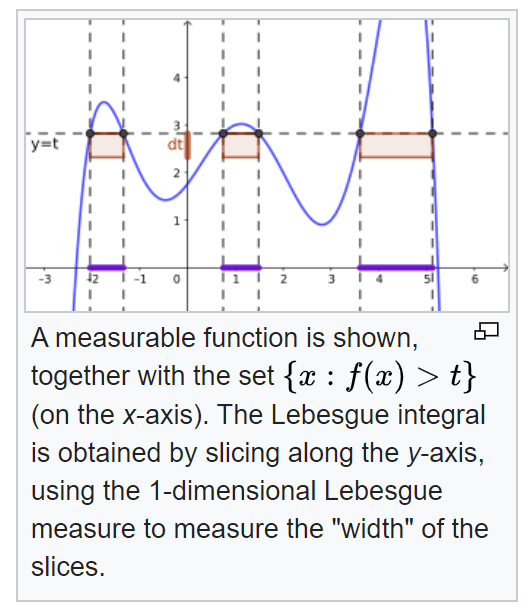
\includegraphics[width=7cm]{img/leb1.png}
    \caption{}
    \label{fig:leb1}
\end{figure}
An equivalent way to introduce the Lebesgue integral is to use so-called simple functions, which generalize the step functions of Riemann integration. Consider, for example, determining the cumulative COVID-19 case count from a graph of smoothed new daily cases (Fig. \ref{fig:leb2}). 
\begin{itemize}
    \item[*]\textbf{The Riemann–Darboux approach}
    \\Partition the domain (time period) into intervals (eight, in the example at right) and construct bars with heights that meet the graph. The cumulative count is found by summing, over all bars, the product of interval width (time in days) and the bar height (cases per day).
    \item[*]\textbf{The Lebesgue approach}
    \\Choose a finite number of target values (eight, in the example) in the range of the function. By constructing bars with heights equal to these values, but below the function, they imply a partitioning of the domain into the same number of subsets (subsets, indicated by color in the example, need not be connected). This is a "simple function," as described below. The cumulative count is found by summing, over all subsets of the domain, the product of the measure on that subset (total time in days) and the bar height (cases per day).
\end{itemize}

\begin{figure}[h]
    \centering
    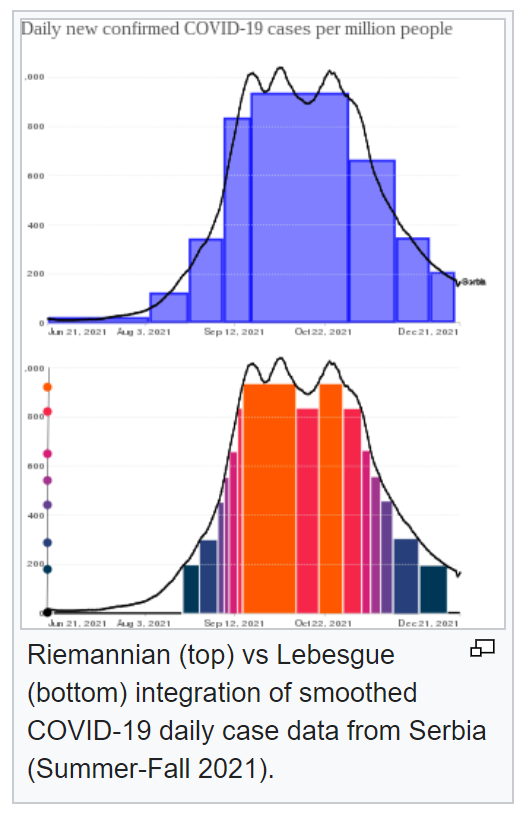
\includegraphics[width=7cm]{img/leb2.png}
    \caption{}
    \label{fig:leb2}
\end{figure}

Let's now go back to the mathematics and give a rigorous formulation of the Lebesgue integral.\\
Let $\mathscr{B}(\rb)$ denote the $\sigma$-algebra of Borel subsets of $\rb$. This is the $\sigma$-algebra generated by all open subsets of $\rb$ and is also generated by the collection of all intervals, or by the collection of all intervals of the form $(c, \infty)$. 
\\Let $(X, \mathscr{B}, m)$ a measure space. A function $f: X \rightarrow \rb$ is \textit{measurable} if $f^{-1}(D) \in \mathscr{B}$ whenever $D \in \mathscr{B}(\rb)$ or equivalently if $f^{-1}(c, \infty) \in \mathscr{B}$ for all $c \in \rb$. A function $f: X \rightarrow \mathbb{C}$ is measurable if both its imaginary and real part are measurable. We say $f=g$ \textit{almost everywhere} (a.e.) if $m\big( 
\{ x: f(x) \neq g(x) \} \big) = 0$, i.e. the functions have equal values everywhere except for a set which has null measure.\footnote{If the only open set of zero measure in a topological space $X$ is the void set, then being equal a.e. for $f$ and $g$ implies being equal. } In measure theory, all sets of null measure are "invisible". 
\\Let $(X, \mathscr{B}, m)$ be a probability space. A function $f: X \rightarrow \rb$ is a \textit{simple function} if it can be written in the form $\sum_{i=1}^n a_i \chi_{A_i}$, where $a_i \in \rb$, $A_i \in \mathscr{B}$, the sets $A_i$ are disjoint sets of $X$, and $\chi_{A_i}$ denotes the characteristic function of $A_i$ ($\chi(x) = 1$ if $x \in A_i$, $0$ otherwise). Simple functions are measurable. We define the integral for simple functions by:
\begin{equation}
    \label{eq:simple_functions_integral}
    \int f \, dm = \sum_{i=1}^n a_i m(A_i) \, .
\end{equation}
This value is independent of the representation $\sum_{i=1} a_i \chi_{A_i}$.  
\\Suppose $f: X \rightarrow \rb$ is measurable and $f \geq 0$. Then there exists an increasing sequence of simple functions $f_n \rightarrow f$. For example, we could take
\begin{equation*}
    f_n(x) = 
    \begin{cases}
        \frac{i-1}{2^n}, \:& \text{if} \, \frac{i-1}{2^n} \leq f(x) \leq \frac{i}{2^n} \: i = 1, \dots, n2^n \\
        n, & \text{if} \, f(x) \geq n \, .
    \end{cases}
\end{equation*}
We define $\int f \, dm = \lim_{n \rightarrow \infty} \int f_n \, dm$ and note that this definition is independent of the chosen sequence $\{ f_n \}$. We say $f$ is \textit{integrable} if $\int f \, dm < \infty$. 
\\Suppose $f:X \rightarrow \rb$ is measurable. Then $f = f^+ - f^-$ where $f^+(x) = \max \{f(x), 0 \} \geq 0$ and $f^- = \max \{ -f(x), 0 \} \geq 0$. We say that $f$ is integrable if $\int f^+ dm$, $\int f^- dm < \infty$ and we then define 
\begin{equation*}
    \int f \, dm = \int f^+ dm - \int f^- dm
\end{equation*}
Notice that $f$ is (Lebesgue-)integrable if and only if $|f|$ is integrable. If $f=g$ a.e. then one is integrable if the other is and $\int f \, dm = \int g \, dm$. 
\\The main theorems on integrating sequences as functions are the following: 
\begin{theorem}[Dominated Convergence Theorem]
Suppose $f_1 \leq f_2 \leq f_3 \leq \dots$ is an increasing sequence of integrable real-valued functions on $(X, \mathscr{B}, m)$. If $\big\{ \int f_n \, dm \big\}$ is a bounded sequence of real numbers, then $\lim_{n \rightarrow \infty} f_n$ exists a.e. and is integrable and $\int (\lim_{n \rightarrow \infty} f_n) dm = \lim_{n \rightarrow \infty} \int f_n$. If instead $\big\{ \int f_n \, dm \big\}$ is an unbounded sequence then either $\lim_{n \rightarrow \infty} f_n$ is infinite on a set of not zero measure or $\lim_{n \rightarrow \infty} f_n$ is not integrable. 
\end{theorem}
\begin{lemma}[Fatou's Lemma]
Let $\{ f_n \}$ be a sequence of measurable real-valued functions on $(X, \mathscr{B}, m)$ which is bounded below by an integrable function. If $\liminf_{n\rightarrow\infty} \int f_n \, dm < \infty$ then $\liminf_{n\rightarrow\infty} f_n$ is integrable and $\int 
 \liminf_{n\rightarrow\infty} f_n \, dm \leq \liminf_{n\rightarrow\infty} \int f_n \, dm$
 \end{lemma}
 
\begin{corollary}[Dominated Convergence Theorem]
 If $g:X \rightarrow \rb$ is integrable and $\{ f_n \}$ is a sequence of measurable real-valued functions with $|f_n| \leq g$ a.e. and $\lim_{n\rightarrow\infty} f_n = f$ a.e. then f is integrable and $\lim_{n\rightarrow\infty} \int f_n \, dm = \int f \, dm$. 
 \end{corollary}
We denote by $L^1(X)$ the space of all Lebesgue integrable functions. Such space is a Banach space with norm $\|f\|_1 = \int |f| \, dm$. If $f \in L^1(X)$, then $\int_A f \, dm$ denotes $\int f \cdot \chi_A \, dm$. 

\section{Perron-Frobenius Theory}
\label{par:perron_frobenius_theory}
In matrix theory, the Perron–Frobenius theorem, proved by Oskar Perron $(1907)$ and Georg Frobenius $(1912)$, asserts that a real square matrix with positive entries has a unique largest real eigenvalue and that the corresponding eigenvector can be chosen to have strictly positive components, and also asserts a similar statement for certain classes of non-negative matrices.
\\This theorem has important applications to probability theory (ergodicity of Markov chains); to the theory of dynamical systems (subshifts of finite type); to economics (Okishio's theorem, Hawkins–Simon condition); to demography (Leslie population age distribution model); to social networks (DeGroot learning process); to Internet search engines (PageRank); and even to ranking of football teams.
\\Let $A=[a_{ij}]$ be a $k \times k$ matrix. We say $A$ is non-negative if $a_{ij} \geq 0$ for all $i,j$. Such a matrix is called \textit{irreducible} if for any pair $i,j$ there is some $n>0$ such that $a_{ij}^{(n)}>0$ where $a_{ij}^{(n)}$ is the $(i,j)$-th element of $A^n$. The matrix $A$ is \textit{irreducible} and \textit{aperodic} if there exists $n>0$ such that $a_{ij}^{(n)} >0$ for \textit{all} $i,j$. We shall use the following result:
\begin{theorem}[Perron-Frobenius Theorem]
    Let $A = [a_{ij}]$ be a non-negative $k \times k$ matrix. Then:
    \begin{itemize}
        \item[(i)] There is a non negative eigenvalue $\lambda$ such that no eigenvalue of $A$ has absolute value greater than $\lambda$.
        \item[(ii)] We have $\min_i( \sum_{j=1}^k a_{ij}) \leq \lambda \leq \max_i( \sum_{j=1}^k a_{ij})$
        \item[(iii)] Corresponding to the eigenvalue $\lambda$ there is a non-negative left (row) eigenvector $u = (u_1, \dots, u_k)$ and a non-negative right (column) eigenvector
        \begin{equation*}
        v = 
            \begin{pmatrix}
                v_1 \\
                \vdots \\
                v_k
            \end{pmatrix}
        \end{equation*}
        \item[(iv)] If $A$ is irreducible then $\lambda$ is a simple eigenvalue and the corresponding eigenvectors are strictly positive (i.e. $u_i >0$, $v_i >0$ $\forall i$).
        \item[(v)] If $A$ is irreducible then $\lambda$ is the only eigenvalue of $A$ with a non-negative eigenvector.
    \end{itemize}
\end{theorem}
This result, as already said, will become very useful when we'll talk about Markov Chain and Hidden Markov Models.


\chapter{Basics of ergodic information theory}

\section{Stochastic processes and properties of the measure}
We can now go back to the discussion in \cref{par:measure_spaces} and state some useful and insightful results.
\\First of all, recall that we are dealing now with the space of all infinite sequences of our finite alphabet, $\Omega = \mathcal{A}^{\nb}$. We introduced earlier a measure $\mu$ on this space and defined the marginals of our measure as the functions $\mu\big( [x_1^n] \big) = \mu(x_1 ,\dots, x_n, \dots) \equiv \mu_n$ acting on the so called canonical cylinders. Most of the time, we will be working with the so called \textit{stochastic processes}.
\begin{definition}[Stochastic Process]
    A stochastic process is an infinite sequence $X \equiv \big\{ X_n \big\} = \big\{ X_1, X_2, \dots, X_n, \dots \big\}$ of random variables $X_n$ with values in $\alp$, defined by the $k-$th order joint distribution on $\alp^k$:
    \begin{equation*}
        \mu_k(a_1^k) \equiv \mathbb{P} \big( X_1^k = a_1^k \big) \, , \quad a_1^k \in \alp^k
    \end{equation*}
\end{definition}
Equivalently, the distribution of a stochastic process can be completely defined by means of the conditional probabilities, by starting from the one-character distribution $\mu_1$ and then computing the successive conditional distributions:
\begin{equation}
    \mu(x_n|x_1^{n-1}) = \frac{\mu_n(x_1^n)}{\mu_{n-1}(x_1^{n-1})}
\end{equation}
since we could iterate the formula to get 
\begin{equation*}
    \mu(\omega_1, \dots, \omega_n) = \mu(\omega_1) \mu(\omega_2|\omega_1)\mu(\omega_3|\omega_2\omega_1) \dots \mu(\omega_k|\omega_1 \dots \omega_{k-1}) \dots \mu(\omega_n|\omega_1 \dots \omega_{n-1}) 
\end{equation*}
The process $\mu$ is said to be \textbf{\textit{stationary}} if 
\begin{equation}
    \mu(x_1^k) = \mu(x_{n+1}^{n+k}) \: \forall a \in \alp
\end{equation}
We can consider now some dynamics on our probability space $(\Omega, \mathscr{B}, \mu)$, i.e. we consider a transformation $T: \Omega \longrightarrow \Omega'$, where $(\Omega', \mathscr{B}', \mu')$ is another probability space. Most of the times we will actually consider simply consider $\Omega' = \Omega, \mu' = \mu, \mathscr{B}' = \mathscr{B}$. 
\\A transformation $T: \Omega \longrightarrow \Omega'$ is said to be \textit{measurable} if $T^{-1}(\mathscr{B}') \subset \mathscr{B}$ (i.e. $B' \in \mathscr{B}' \Rightarrow T^{-1}B' \in \mathscr{B}$).
\\A transformation $T: \Omega \rightarrow \Omega$ is \textit{measure preserving} if $\forall A \in \mathscr{B}$ we have $\mu \big( T^{-1}(A) \big) = \mu(A)$. We equivalently say then that $T$ is measure preserving or that $\mu$ is \textit{$T$-invariant}, so that $\mu \circ T^{-1} = \mu$. $\mu \circ T^{-1}$ is sometimes referred to as the "pull-back measure" $T^* \mu$. Since $\Omega$ is compact, we can consider the set of all measures on $\Omega$, 
\begin{equation}
    \mathcal{P} = \big\{ \mu \big| \, \mu \, \text{is a finite measure w/} \, \mu(\Omega) = 1 \big\}
\end{equation}
and also we can define 
\begin{equation}
    \mathcal{P}_I = \big\{ \mu \in \mathcal{P} \big| \, \mu \circ T^{-1} = \mu \big\}
\end{equation}
as the collection of all invariant measures (depending on the dynamics). 
\\There is a natural dynamics on $\Omega$: consider $x= (x_0,x_1, \dots, x_n, \dots), x_j \in \alp$. The \textit{\textbf{shift}} is defined as:
\begin{gather}
    \sigma: \Omega \longrightarrow \Omega\nonumber \\
    \sigma : (x_0,x_1, \dots, x_n, \dots) \longrightarrow (x_1, x_2, \dots, x_n, \dots) 
\end{gather}
Its name should be self explicative: it shifts the sequences (to the left).
\\A \textbf{\textit{process}} or a \textbf{\textit{source}} is a shift-invariant probability measure $\mu$ on the topological space $\alp^{\zb}$. The process is uniquely defined by the joint distribution, and not really by the exact values of the $x_n$'s. 
 The shift is closely related to the property of stationarity of the measure: actually, both properties are equivalent.
\begin{prop}[$\sigma$-invariancy $\Leftrightarrow$ stationarity]
Shift invariance implies stationarity, and viceversa. 
\end{prop}
\begin{proof}
    By definition, $\sigma^{-1}( [x_1^n] ) = \{ z \in \Omega \big| \sigma(z) \in [x_1^n] \} = \bigsqcup_{a \in \mathcal{A}} [a, x_1, \dots, x_n]$.
    Then the proof is straightforward, since
    \begin{equation*}
        \mu(\sigma^{-1}( [x_1^n])) = \mu( [x_1^n]) = \sum_{a \in \mathcal{A}} \mu(a, x_1, \dots, x_n)
    \end{equation*}
\end{proof}
Now we may ask ourselves: what if we take $\mu_{n+1} = \mu\big( [x_1{n+1}] \big)$? What is its measure? Notice that 
\begin{equation*}
    [x_1^n] = \bigsqcup_{a \in \mathcal{A}} (x_1, \dots, x_n, a) \, ,
\end{equation*}
i.e. the disjoint union of all sequences which have an arbitrary $n+1$ letter. Thus we can now state the \textit{consistency relations} (or \textit{compatibility conditions}):
\begin{prop}[Consistency relations]
\label{prop:consistency_rel}
\hfill
\\$\mu$ is a measure on $\Omega$ iff:
    \begin{itemize}
        \item[(1)] $\sum_{a_1, \dots, a_k \in \alp} \mu_k(a_1, \dots, a_k) = 1$
        \item[(2)] $\mu_n(x_1, \dots, x_n, \dots) = \sum_{a \in \mathcal{A}} \mu_{n+1} ((x_1, \dots, x_n, \dots, a)$
    \end{itemize}
iff $\mu$ is shift invariant, 
    \begin{itemize}
        \item[(3)] 
         $\mu_n(x_1, \dots, x_n, \dots) = \sum_{a \in \alp} \mu_{n+1}(a, x_1, \dots, x_n, \dots)$
    \end{itemize}
\end{prop}
We can now state a very important result:
\begin{theorem}[Kolmogorov representation theorem]
    If $\{ \mu_k \}$ is a sequence of measure defining a process then there is a \textbf{unique} probability measure $\mu$ on $\alp^{\nb}$ such that, for each $k \geq 1$ and for each cylinder $x_1^k$
    \begin{equation*}
        \mu\big( [x_1^k] \big) = \mu_k(x_1^k)
    \end{equation*}
\end{theorem}
Basically, this is telling us that not only we can reconstruct the measure from the marginals, but that such measure will be the only one we can define on $\Omega$ given such marginals.

\section{Examples of invariant measures}
Let's see some basic examples of invariant measures.
\subsection{i.i.d. (independent identically distributed variables)}
Assume that we have a set of measures $p_1,p_2, \dots, p_n$ over $\alp$ such that 
\begin{gather}
    p_k : \alp \longrightarrow \rb^+ \nonumber \\ 
    p_k \geq 0 \nonumber \\
    \sum_{a \in \alp} p_k(a) = 1 \quad \forall k 
\end{gather}
Define then 
\begin{equation}
    \mu_n(x_1^n) = \mathbb{P}(x_1, \dots, x_n) = \prod_k p_k(x_k)
\end{equation}
choosing $x_1$ with probability $p_1$, $x_2$ with probability $p_2$ and so on. These marginals satisfy all three conditions; consider the first one for example:
\begin{equation*}
    \sum_{x_{n+1}}\mu(x_1 , \dots, x_{n+1}) = p_1(x_1) p_2(x_2) \dots p_n(x_n) \bigg[ \sum_{x_{n+1}} p_{n+1} (x_{n+1}) \bigg] = \mu(x_1 , \dots, x_n)
\end{equation*}
\textit{exercise:} prove that $\forall p_1, \dots, p_n$:
\begin{itemize}
    \item[i)] $\mu = \bigotimes_{j=1}^{\infty}p_j \in \mathcal{P}(\Omega)$
    \item[ii)] $\mu \in \mathcal{P}_I(\Omega) \Leftrightarrow p_k = p : \alp \rightarrow \rb^+ \, \forall k$
\end{itemize}
\subsection{Markov processes}
Markov processes are the easiest stochastic processes with memory. Their definition is quite straightforward:
\begin{definition}[Markov of order $k$]
    \hfill \\
    A process is said to be Markov of order $k$ if
    \begin{equation}
        \mathbb{P}(x_n = a_n \big| x_1^{n-1}) = \mathbb{P}(x_n = a_n \big| x_{n-k}^{n-1}) , \quad n>k
    \end{equation}
    A Markov process of order $1$ is called a Markov chain, i.e. a process is a Markov chain if 
    \begin{equation}
         \mathbb{P}(x_n = a_n \big| x_1^{n-1}) = \mathbb{P}(x_n = a_n \big| x_{n-1}) 
    \end{equation}
\end{definition}
Markov processes have been studied in the past decades to a great extent. We can completely describe a Markov process. To do such thing we have to introduce some objects which simplify our description.
\\First of all, let $\alp = \big\{ a_1, \dots, a_l \big\}$ be our alphabet, with $|\alp| = l$. In a Markov process, the $a_k$'s are called \textit{states}. Consider then a probability vector 
\begin{gather}
    p = (p_1, \dots, p_l) \nonumber \\
    p_j \geq 0 \, , \, \sum_{j=1}^l p_j = 1
\end{gather}
Let then $P = [p_{ij}]$ be a \textit{stochastic} $l \times l$ \textit{matrix} , i.e.
\begin{gather} 
\label{eq:stochastic_matrix}
    P_{ij} \geq 0 \nonumber \\
    \sum_j P_{ij} = 1 \quad \forall j
\end{gather}
The elements of such matrix represent the probability that from a state $i$ we will transition to a state $j$ in the next iteration of our system, i.e. is a matrix representing transition probabilities. That is why the second condition in eq. (\ref{eq:stochastic_matrix}) exists: it is telling us that the probability to transition from a state $i$ to any of the other states $j$ should be $1$.
\\It can be proven that if $P$ is stochastic, then it has an invariant vector $\vec{1}$ of all ones
\begin{equation*}
    P \vec{1} = 
    \begin{pmatrix}
        1 \\
        1 \\
        \vdots \\
        1
    \end{pmatrix}
\end{equation*}
The Perron-Frobenius theorem \cref{par:perron_frobenius_theory} tells us then that all other eigenvalues are contained in a circle of radius $1$. 
\\A Markov process is thus defined by a couple $\big( p, P \big)$. $p$ is invariant if it is a left-eigenvalue
\begin{equation*}
    p P = p \quad (\Leftrightarrow P^T p = p)
\end{equation*}
What measure should we use for a Markov process? A natural definition is, $\forall n$, $ \forall x_1, \dots, x_n $, would be 
\begin{equation}
\label{eq:markov_measure}
    \mu_n(x_1, \dots, x_n) \equiv p(x_1) \cdot P_{x_1 x_2} \cdot P_{x_2 x_3} \cdots P_{x_{n-1} x_n} 
\end{equation}
\begin{prop}
    The measure $\mu$ defined by such marginals satisfies all the consistency relations \ref{prop:consistency_rel}
\end{prop} 
\begin{proof}
\hfill 
    \begin{itemize}
        \item[i)] From their definition (\ref{eq:markov_measure}), $\forall (x_1, \dots, x_n) \in \alp^n$ we have $\mu_n \geq 0$; also since $p$ is a probability vector and $P$ a stochastic matrix we will have $\forall n$ that $\sum_{(x_1, \dots, x_n) \in \alp^n} \mu_n (x_1, \dots, x_n) = 1 $ 
        \item[ii)] The second property $\sum_{x_{n+1}} \mu_{n+1} (x_1, \dots, x_{n+1}) = \mu_n (x_1, \dots, x_n)$ also follows from the definition (\ref{eq:markov_measure}) and stochasticity of $P$
        \item[iii)] The only thing left to prove is that $\sum_{x_0} \mu_{n+1} (x_0, x_1, \dots, x_n) =  \mu_n (x_1, \dots, x_n)$. This is actually straightforward since 
        \begin{equation*}
            \sum_{x_0} p_{x_0} P_{x_0 x_1} P_{x_1 x_2} \cdots P_{x_{n-1} x_n} = p(x_1) P_{x_1 x_2} \cdots P_{x_{n-1} x_n}
        \end{equation*}
        where we used the fact that $p$ is an eigenvector of $P$ and thus $(pP)_{x_1} = p_{x_1}$
    \end{itemize}
\end{proof}
By Kolmogorov we then know that this is the unique invariant measure we can define on a Markov process $(p, P)$.
\\An interesting and useful fact is that a markov of order $k$ can always be reduced to order $1$ by using a bigger alphabet (whose cardinality grows exponentially though, so that this becomes difficult to implement in concrete problems). Let's consider for example a Markov of order $2$, 
\begin{equation*}
    \mu (x_1, \dots, x_n \big| x_{n+1}) = \mu (x_1, \dots, x_n) \mu (x_{n+1} \big| x_1, \dots, x_n) = \mu (x_1, \dots, x_n \big| x_{n+1}x_n)
\end{equation*}
Now consider 
\begin{equation*}
    \alp^{(2)} = \big\{ a_ja_k \equiv b \big| 
    \begin{matrix}
        a_j \in \alp \\
        a_k \in \alp
    \end{matrix}
    \big\}
\end{equation*}
as the set of all bigrams. Of course if $\mu$ is a Markov of order $2$ on $\alp$ it can be seen as a Markov Chain on $\alp^{(2)}$.
\\Consider now a Markov chain over $\alp$ with $|\alp| = l$; it may happen that some elements of $P$ are zero, for example consider
\begin{gather*}
    p_j > 0 \quad j=1, \dots, k \\
    p(a_j) = 0 \quad j=k+1, \dots, l
\end{gather*}
we can then reduce this to a Markov chain over $\alp^k$, a smaller alphabet, just erasing rows and column of $P$ to get a new $\hat{P}$ which will be $k \times k$, 
\begin{equation*}
    (p,P) \, \, \text{on} \, \, \alp^l \longrightarrow (\hat{p},\hat{P}) \,\, \text{on} \,\, \alp^k
\end{equation*}

\subsection{Hidden Markow Models}
A hidden Markov model (HMM) is a statistical Markov model in which the system being modeled is assumed to be a Markov process with unobservable ("hidden") states.
\\Let's consider two alphabets: 
\begin{align}
    &\alp = \big\{ x_1, \dots, x_n \big\} \quad \text{observable states} \nonumber \\
    &\mathcal{L} = \big\{ y_1, \dots, y_l \big\} \quad \text{hidden states}
\end{align}
We assume that there exists a rectangular stochastic matrix $R$ such that
\begin{gather}
    R = [R_{yx}]_{y \in \mathcal{L}, \, x \in \alp} \nonumber \\
    \sum_{x \in \alp} R_{yx} = 1 \quad \forall y \in \mathcal{L}
\end{gather}
The elements of $R$ represent the so called \textit{emission probabilities}, i.e. the probabilities to go from an hidden state $y \in \mathcal{L}$ to an observable state $x \in \alp$. Summing on all observable states should amount to $1$ since from an hidden state we must go to some observable state sooner or later (see Fig. \ref{fig:HMM1}). 
\\Surely, we must also assume that there exists also a stochastic matrix for the hidden states with their transition probabilities: this would be the $l \times l$ matrix $P = [P]_{y z}$ $\forall y,z \in \mathcal{L}$. We shall also consider a probability vector $p$ for this Markov system. An HMM is thus defined by a triplet $\big(p, P, R \big)$
\\Then we define the measure for this system as 
\begin{equation}
    \mu_n (x_1, \dots, x_n) = \sum_{(y_1, \dots, y_l) \in \mathcal{L}} p_{y_1} R_{y_1 x_1} P_{y_1 y_2} R_{y_2 x_2} \cdots P_{y_{n-1} y_n} R_{y_n x_n}
\end{equation}
\textit{exercise}:
\begin{itemize}
    \item[i)] prove that $\mu_n$ are marginals (they statisfy the first $2$ consistency relations)
    \item[ii)] prove that if $pP=p$ then $\mu$ is invariant 
\end{itemize}
There is an equivalent way of defining such measure: we can consider the matrix $M_x$ $\forall x \in \alp$ defined as 
\begin{equation}
    M_x = [m_{yz}^{(x)}]_{y, z \in \mathcal{L}} = \big[ R_{yx} P_{yz} \big]
\end{equation}
so that $P = \sum_{x \in \alp} M_x$. These are again $l \times l$ matrices, and there are $n = |\alp|$ of them.
\\This gives us an equivalent representation of an HMM, since considering a probability vector $p = (p_1, \dots, p_l)$ we can define the marginals as 
\begin{equation}
    \mu_n (x_1, \dots, x_n) \equiv p M_{x_1} M_{x_2} \cdots M_{x_n} \cdot 
    \begin{pmatrix}
        1 \\
        1 \\
        \vdots \\
        1
    \end{pmatrix} 
    \,\, \geq 0
\end{equation}

\begin{figure}[h]
    \centering
    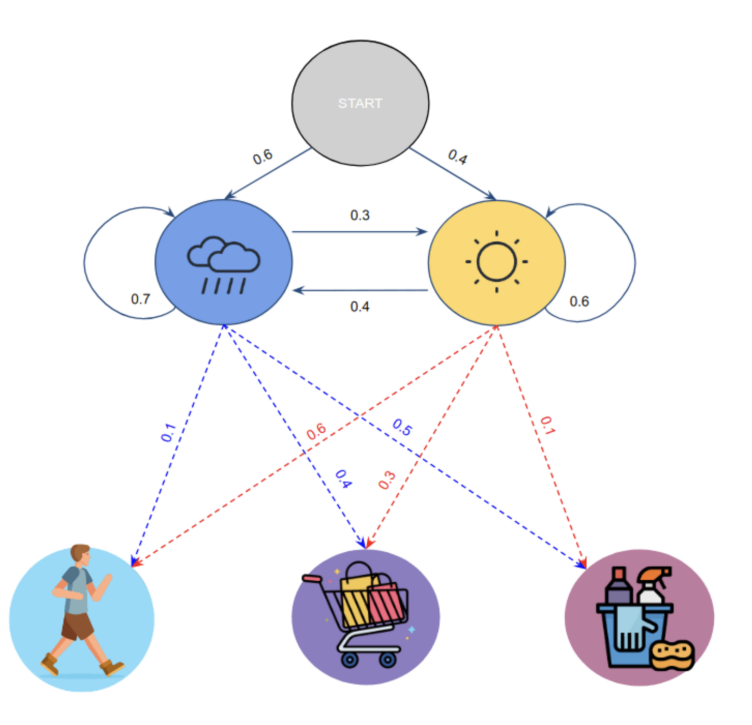
\includegraphics[width=7cm]{img/HMM1.png}
    \caption{Schematic representation of an Hidden Markov Model. My friend lives in the States. Depending on the weather there, he chooses the activity he does every day. I am not able to know the weather where he lives (hidden states), I only know what he is doing that day (observable states).}
    \label{fig:HMM1}
\end{figure}

\section{Ergodic Theory}
We shall now look at some basics results of Ergodic Theory.
\\Consider a space $\man$ with a measure $\mu$ and a certain dynamic $T$ which is measure preserving. Such transformation could be either discrete or continuous (a so called \textit{flow} $\Phi^t$). Given an $x_0 \in \man$ we are interested in studying the orbit under $T$, i.e. all the points $\mathcal{O}(x) = \big\{ x \in \man \big| \, x_n = T^n(x_0), \, \forall n \in \nb \big\}$. 
\\The first thing that comes natural to study are functions from $\man $ to $\rb$, out \textit{observables} $f: \man \longrightarrow \rb$. 
\\We are interested in knowing the asymptotic statistical properties of such observables, i.e. we would like to know for each $f$ what happens to the average
\begin{equation*}
    \lim_{n \rightarrow \infty} \frac{f(x_0) + f(x_1) + \dots + f(x_n)}{n} = \lim_{n \rightarrow \infty} \frac{1}{n} \sum_{k=0}^{n-1} f \circ T^k(x) \equiv f^*(x)
\end{equation*} 
\begin{remark}
    equivalently for flows we could consider 
    \begin{equation}
        \frac{1}{T} \int_0^T (f \circ \Phi^t) (x) \, d\mu
    \end{equation}
    and then take the limit for $T \rightarrow \infty$
\end{remark}
Let's then define the spatial mean of a function $f$, if it exists, as 
\begin{equation}
    \Bar{f} = \int_{\man} f(x) \, d\mu
\end{equation}
A very important classical result is Birkhoff Ergodic Theorem.
\begin{theorem}[Birkhoff Ergodic Theorem]
    Let $(\man, T, \mu)$ be a dynamical system, and $f \in L^1 \big( \man, \mu \big)$ a summable function with complex values. Then 
    \begin{itemize}
        \item[a)] $f^* (x)$ exists $\mu$-almost everywhere
        \item[b)] $f^* (x)$ is summable and invariant almost everywhere, i.e. 
        \begin{equation*}
            f^* (T^k (x) ) = f^*(x) \quad \forall k \, \, \text{a.e.}
        \end{equation*}
        \item[c)] 
        \begin{equation*}
            \int_{\man} f^*(x) \, d\mu = \int_{\man} f \, d\mu
        \end{equation*}
    \end{itemize}
\end{theorem}
Let's define a particular class of functions which will be very useful:
\begin{definition}[Characteristic functions]
    The characteristic function of an open set $A \in \man$ is defined as 
    \begin{equation}
    \chi_A (x) = 
        \begin{cases}
            1 \quad & \text{if} \quad x \in A \\
            0 \quad & \text{if} \quad x \notin A
        \end{cases}
    \end{equation}
\end{definition}
\textit{exercise:} prove that $\chi_A \circ T = \chi_{T^{-1}(A)}$, $\, \forall x \in \man$. 
\begin{prop}
    The following are equivalent:
    \begin{itemize}
        \item[a)] $\forall f \in L^1$, $f^*=c$ $\mu-$a.e.
        \item[b)] $\forall f \in L^1$, $f^*= \int_{\man} f \, d\mu = \Bar{f}$
        \item[c)] if $f \in L^1$ is invariant $\Rightarrow f=$constant
        \item[d)] if $A \subseteq \man$, $A$ measurable and invariant $\Rightarrow \mu(A) = 0,1$
    \end{itemize}
\end{prop}
\begin{proof}
\hfill
    \begin{itemize}
        \item a) $\Rightarrow$ b): \\
         if $f \in L^1$ then $\Rightarrow f= $ constant by a). By point $b$ of Birkoff's theorem we have then 
         \begin{equation*}
             \int_{\man} c \, d\mu =\int_{\man} f^* \, d\mu = \int_{\man} f \, d\mu
         \end{equation*}
         \item b) $\Rightarrow$ c): \\
         take $f$ to be invariant, i.e. $f \circ T = f$: then $f \circ T^k = f \, \forall k \in \nb \Rightarrow f^* = f$
         \item c) $\Rightarrow$ d): \\
         Apply c) to $f = \chi_A \in L^1$. Since $T^{-1}A = A$ mod$\mu$ $\Rightarrow \chi_{T^{-1}A} = \chi_A$ then we have by c) that $\chi_A =$const. By the definition of $\chi$ then we must have const$=0$ and $A = \emptyset$ or const$=1$ and $A = \man$.
         \item d) $\Rightarrow$ a): \\
         claim : $f: \man \rightarrow \rb$ is constant a.e. iff $\nexists l \in \rb$ such that $\mu( \{ x \in \man | f(x) = l \} ) \in (0,1)$, meaning that we only want $\mu$ to have a single jump from $0$ to $1$ and not multiple jumps.
         \\Consider now $f^*$. Suppose that $\nexists l \in \rb$ s.t. for $A_l = \{ x \in \man | f^*(x) = l \}$ s.t. $\mu (A_l) \in (0,1)$. Clearly $T^{-1}A_l = A_l$. But then 
         \begin{equation*}
             T^{-1}A_l = \{ y \in \man | \, f^* (Ty) \leq l \} = A_l \Rightarrow f^* (Ty) = f^*(y)
         \end{equation*}
         and we get a contradiction.
    \end{itemize}
\end{proof}
Thus ergodicity of a system can be also seen as the \textbf{equivalence of time mean and phase space means} of an observable (which is what Boltzmann had hoped was true for any dynamical system). 
\\We can also say that 
\begin{equation*}
     \text{$\%$ of time spent by $\mathcal{O}(x)$ in $A$} =  \frac{ \# \big\{ k | \, x_k \in A \big\}}{n} \xrightarrow{n \rightarrow \infty} \mu(A) = \frac{\mu(A)}{\mu(\man)}  
\end{equation*}
This follows directly from Birkoff's theorem, since if we consider $\chi_A (x)$ then we'll have 
\begin{equation*}
    \chi^*_A = \lim_{n \rightarrow \infty} \frac{1}{n} \sum_{k=0}^{n-1} \chi_A \circ T^k(x) = \int_{\man} \chi_A \, d\mu
\end{equation*} 
Therefore, \textbf{in an ergodic system all orbits visit volumes in phase space for a time proportional to the volumes themself}. \\
Now we could ask ourselves: how does all the discussion about infinite sequences of finite alphabets relate to ergodic theory and its application? The key to deeply connect both arguments will be \textit{partioning}. 
\\Given our measurable dynamical system $(X, \mu, T)$, consider $X$ as partitioned in disjoint sets $P_a$ indexed by a finite alphabet $\alp$, i.e. consider a finite partition $\mathcal{P}$ of $X$ such that
\begin{gather}
    \mathcal{P} = \big\{ P_a \big\}_{a \in \alp} \nonumber \\
    X = \bigsqcup_{a \in \alp} P_a
\end{gather}
The $P_a$'a only intersect on boundaries (sets of zero measure) as shown in Fig. \ref{fig:partition} 
\begin{figure}[h]
    \centering
    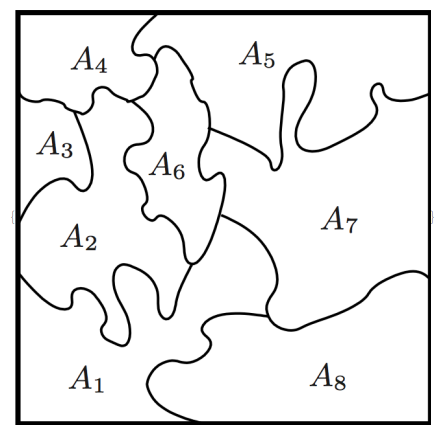
\includegraphics[width=5cm]{img/partition.png}
    \caption{Schematic depiction of a partition of a manifold $X$.}
    \label{fig:partition}
\end{figure}
Then associate each iteration of the dynamics $x_j = T^J(x_0)$ with a given symbol of $\alp$ by the map
\begin{gather*}
    x_1 \longrightarrow \omega_1 \\
    x_2 \longrightarrow \omega_2 \\
    \vdots \\
    x_n \longrightarrow \omega_n \\
    \vdots \\
    \text{where} \quad x_j \in P_{\omega_j}
\end{gather*}
This allows us to equivalently consider an orbit $\mathcal{O}(x)$ or a sequence of characters from our alphabet. 
\\But what measure should we use for such sequences? A marginal $\mu_k(\omega_1^k)$ will now measure all the points which are in $P_{\omega_1}$ at $t_1$, $P_{\omega_2}$ at $t_2$ and so on ($\omega_1$ and $\omega_2$ possibly being the same symbol). Let's define then
\begin{equation}
\label{eq:measure_partition}
    \mu_k (\omega_1^k) = \mu \big( \bigcap_{j=1}^k T^{-j+1} P_{\omega_j} \big)
\end{equation}
\textit{exercise:} prove that such $\mu_k$'s are in fact marginals and that the transformation $T$ commutes with the shift $\sigma$ and that $\mu$ is then $\sigma$- invariant.
\begin{definition}
    The (stationary) process $\{ X_n \}_{n \in \nb}$ defined by the measure (\ref{eq:measure_partition}) is called a $(T, \mathcal{P})$-process
\end{definition}
We can now finally move on to the definition of ergodicity. This comes very naturally by the setting we are now working in. First of all, let's see a couple of definitions needed to state ergodicity:
\begin{definition}
    A measurable set $B \in X$ is said to be $T$-invariant if $TB \subseteq B$
\end{definition}
\begin{definition}
    The space $X$ is said to be $T$-decomposable if it can be expressed as the disjoint union $X = X_1 \bigsqcup X_2$ of two measurable invariant\footnote{since the sets are invariant, the orbit of a point in $X_1$ stays in $X_2$ and the same thing happens for $X_2$. Therefore we could study the two subsystem separately} sets, each of positive measure. Hence, the space is indecomposable if 
    \begin{equation*}
        T^{-1}B = B \Rightarrow \mu(B) = 0 \, \vee \, \mu(B) = 1
    \end{equation*}
\end{definition}
This is exactly what we mean for ergodicity. 
\begin{definition}[Ergodicity]
    A measure-preserving tranformation $T$ is said to be \textbf{ergodic} if
    \begin{equation}
        T^{-1}B = B \Rightarrow \mu(B) = 0 \, \vee \, \mu(B) = 1
    \end{equation}
\end{definition}
Thus \textbf{ergodicity of our system means that we cannot subdivide it in smaller parts to study them separately}.
\\Notice that Hamiltonian systems are not ergodic: we can subdivide them in hypersurfaces where the hamiltonian $H=E$ is constant. 
\begin{lemma}[Ergodicity equivalents]
    The following are equivalent for a $\mu$-measure preserving transformation $T$:
    \begin{itemize}
        \item[1)] $T$ is ergodic
        \item[2)] $T^{-1}B \subseteq B \Rightarrow \mu(B) = 0 \, \vee \, \mu(B) = 1$
        \item[3)] $T^{-1}B \supseteq B \Rightarrow \mu(B) = 0 \, \vee \, \mu(B) = 1$
        \item[4)] $\mu (T^{-1}B \Delta B) = 0 \Rightarrow \mu(B) = 0 \, \vee \, \mu(B) = 1$
        \item[5)] $f \circ T = f$ a.e. $\Rightarrow f$ constant a.e.
    \end{itemize}
\end{lemma}
The last claim can be proved by recalling that $\chi_A \circ T = \chi_{T^{-1}A}$ (\textit{exercise}). 
\\We will see later on what ergodicity of our system means in the setting we discussed earlier. Basically, it will coincide with an application of ergodicity itself, which is the convergence of empirical probabilities. But for now, let's stick to studying some other basic results of ergodic theory.
\\Sometimes, to show that a process is ergodic it is even simpler to prove a stronger property, called \textit{mixing}. 
\begin{definition}[Mixing]
    A measure preserving transformation $T$ is mixing if for any pair of measurable sets $C$ and $D$ we have
    \begin{equation}
        \lim_{n \rightarrow \infty} \mu \big( T^{-n}C \cap D \big) = \mu(C) \cdot \mu(D)
    \end{equation}
\end{definition}
This definition is telling us that the fact that a system is mixing corresponds to the fact that correlations are asymptotically decaying\footnote{we could also have "exponential mixing" or "polynomial mixing" based on how the decay evolves with time ($\sim e^{-t}$ or $\sim t^{-\alpha}$)}. Basically then \textit{a mixing system is a system with no memory}. 
\\\textit{exercise:} prove that mixing $\Rightarrow$ ergodicity (and that the viceversa is not true).
\\Actually, some sort of viceversa of mixing $\Rightarrow$ ergodicity does exist, but with looser conditions: we can say that "mixing on average" $\Rightarrow$ ergodicity, in the following sense:
\begin{theorem}
    The dynamical system $(X, \mu, T)$ is ergodic if and only if $\forall A,B \subset X$ 
    \begin{equation}
        \lim_{n \rightarrow \infty} \frac{1}{n} \sum_{j=0}^{n-1} \mu \big( A  \cap T^{-1}B \big) = \mu(A) \cdot \mu(B)
    \end{equation}
\end{theorem}

\subsection{Ergodicity for Markov chains}
When is a Markov chain irreducible? When we cannot have a zero probability to go from a state $j$ to a state $k$.
\begin{definition}[irreducible Markov chains]
    The stochastic matrix $M$ is said to be irreducible if for any pair $j,k$ there is a certain sequence $j_0, j_1, \dots, j_n$ with $j_0=j$ and $j_n=k$ such that each intermediate transition is possible, i.e. 
    \begin{equation}
        M_{j_m j_{m+1}} > 0 \,, \quad m = 0,1, \dots, n-1
    \end{equation}
    Namely, given any pair of states $j$ and $k$, sooner or later strarting from $j$ we'll end up in $k$.
\end{definition}
This actually corresponds (\textit{exercise: chech it}) to the definition of irreducible matrices given in par. \cref{par:perron_frobenius_theory}, i.e. $\forall i,j$ $\exists n = n(i,j) : (P^n)_{ij} > 0$.
If $M$ is irreducible then by Perron-Frobenius (\cref{par:perron_frobenius_theory}) there is a \textbf{unique} probability vector $\pi$ (the \textbf{equilibrium state}):
\begin{equation}
    \pi M = \pi
\end{equation}
i.e. the Markov chain with start distribution $\mu_1=\pi$ and transition matrix $M$ is in fact a stationary process. 
\\Moreover, any initial distribution of characters will \textit{converge to the invariant measure}: given any probability vector $\mu_1$ on $\alp$, we have 
\begin{equation}
    \lim_{n \rightarrow \infty} \mu_1 M^n = \pi
\end{equation}
We can define the equivalent of the mixing property for a Markov chain:
\begin{definition}
    A Markov chain is mixing iff $\exists$ n s.t. $\forall j,k$ we have $M_{jk}^n$.
\end{definition}
This is a stronger requirement than irreducibility, as we are now asking that such $n$ is not a function of the indexes $i,j$ but instead exists for all couples. This definition of mixing is quite straightforward and equivalent to that given before: let's give it a better look. 
\\Consider a Markov system $(p, P)$ on a space $(\Omega=\alp^{\nb}, \mu, T = \sigma)$. Consider then two cylinders $C= [x_1^m]$ and $D= [y_1^r]$. we know that mixing means for our two sets that 
\begin{equation*}
    \lim_{n \rightarrow \infty} \mu (T^{-n}C \cap D) = \mu(C) \, \mu(D)
\end{equation*}
Of course $T^{-n} = \sigma^{-n}$ is just a translation, i.e. $T^{-n}(C) = \big\{ z \in \Omega | \, z_{n+j} = y_j, \quad j=1, \dots, r \big\}$. What is then $T^{-n}C \cap D$? Consider an $n > m$ for simplicity. Then
\begin{equation*}
    T^{-n}C \cap D = \bigg\{ z \in \Omega \bigg| \, 
    \begin{matrix}
        z_1 = x_1 & z_{n+1} = y_1 \\
        \vdots & \vdots\\
        z_m=x_m  & z_{r+n} = y_r
    \end{matrix}
    \bigg\}
\end{equation*}
The measure of this set in with our Markov measure will then be (see Fig. \ref{fig:markov_line}):
\begin{align}
    \mu(T^{-n}C \cap D) = p_{x_1} P_{x_1 x_2} \cdots P_{x_{m-1} x_m} \cdot \bigg( \sum_{z_1, \dots, z_k} P_{z_1 z_2} \cdots P_{z_{t-1} z_t = y_1} \bigg) P_{y_1 y_2} \cdots P_{y_{r-1} y_r} \nonumber \\
    =  p_{x_1} P_{x_1 x_2} \cdots P_{x_{m-1} x_m} \cdot \big( P^t\big)_{x_m y_1} P_{y_1 y_2} \cdots P_{y_{r-1} y_r}
\end{align}
\begin{figure}[h]
    \centering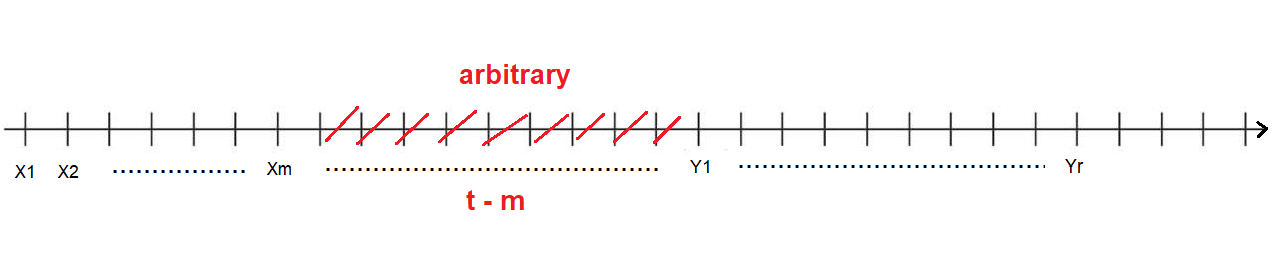
\includegraphics[width=12cm]{img/markov_line.png}
    \caption{Schematic depiction of our Markovian sequences. The sequence from $X_m$ to $Y_1$ is totally arbitrary.}
    \label{fig:markov_line}
\end{figure}
since we must account for all possible paths from $x_m$ to $y_1$ in $t$ steps. 
\\A very useful classical result is the following:
\begin{theorem}[Ergodicity for Markov chains]
\hfill
    \begin{itemize}
        \item[(1)] A stationary Markov chain is ergodic iff its transition matrix $M$ is irreducible
        \item[(2)] If the Markov chain is mixing, then it is ergodic
    \end{itemize}
\end{theorem}
Some more useful results for Markov chains' ergodicity are the following. 
\begin{lemma}{(1.18 in Walter)}
    Let $P$ be a stochastic matrix and $P^n$ its power. Take then a "Birkoff average" of $P$, 
    \begin{equation}
    \label{eq:Q_projector}
        Q = \lim_{n \rightarrow \infty} \frac{1}{n} \sum_{k=0}^{n-1} P^n
    \end{equation}
    Such matrix is a spectral projector, i.e. it satisfies $Q^2 = Q$; moreover, it commutes with $P$, $QP = PQ$ and $\forall v$ such that $vP = v$ we have that $vQ = v$.
\end{lemma}
The existence of $Q$ can be proven by spectral theory. By using $Q$ we can state two theorems which can result useful:
\begin{theorem}
    The following are equivalent:
    \begin{itemize}
        \item[a)] $(\Omega, \mu, T)$ is ergodic;
        \item[b)] $Q$ as defined in (\ref{eq:Q_projector}) is an $l \times l$ matrix of the form 
        \begin{equation*}
            Q = 
            \begin{pmatrix}
                \Vec{p} \\
                \Vec{p} \\
                \vdots \\
                \Vec{p} 
            \end{pmatrix}
        \end{equation*}
        where $p$ is a probability vector (i.e. $pP = p$, $p_j \geq 0$, $\sum_j p_j = 1$)
        \item[c)] $P$ is irreducible
        \item[d)] $\Vec{1}$ s.t. $P \Vec{1} = \Vec{1}$ is a simple eigenvector (but not the only eigenvector).
    \end{itemize}
\end{theorem}
There is an equivalent of the last theorem for mixing:
\begin{theorem}
    The following are equivalent:
    \begin{itemize}
        \item[a)] $(\Omega, \mu, T)$ is mixing;
        \item[b)] $P$ is irreducible and aperiodic
        \item[c)] $P^n \xrightarrow{n \rightarrow \infty} Q$ with 
        \begin{equation*}
            Q = 
            \begin{pmatrix}
                \Vec{p} \\
                \Vec{p} \\
                \vdots \\
                \Vec{p}
            \end{pmatrix}
        \end{equation*}
        \item[d)] $\Vec{1}$ s.t. $P \Vec{1} = \Vec{1}$ is a simple eigenvector \textbf{and} it is the unique eigenvalue on $S^1$ (the circle).
    \end{itemize}
\end{theorem}


\section{Consequences of ergodicity}
\begin{definition}[empirical frequencies]
    Given a sequence $x = x_1^n \in \alp^n$ of length $n$ and a $k$-gram $\omega = \omega_1 \omega_2 \dots \omega_k \in \alp^k$, we define the \textbf{empirical frequency} of the word $\omega$ by 
    \begin{equation}
        f_x(\omega) \equiv | \big\{ j \in [1, n-k+1] : x_j^{j+k-1} = \omega \big\} |
    \end{equation}
\end{definition}
Denoting by $\chi_\omega$ the indicator function of the cylinder $[\omega_1^n]$ we could also write 
\begin{equation}
    f_x(\omega) = \sum_{j=1}^{n-k+1} \chi_\omega (\sigma^{j-1} x)
\end{equation}
Meaning that, since we are looking at how many times a word appears in a sequence, we could do it by sliding a window of size $k$ over our sequence e count a $+1$ for every match. 
\begin{definition}[relative frequency]
    The relative frequency is instead defined as 
    \begin{equation}
        \hat{\mu}_n (\omega_1^k | x_1^n) \equiv \frac{1}{n-k+1} f_x(\omega_1^k)
    \end{equation}
\end{definition}
\begin{definition}[typical sequences]
    A sequence $x \in \alp^{\nb}$ is said to be frequency \textbf{typical} for the process $\mu$ if each word $\omega \in \alp^{\nb}$ appears in $x$ with the statistics predicted by $\mu$, i.e. 
    \begin{equation}
        \lim_{n \rightarrow \infty} \hat{\mu}_n (\omega_1^k | x_1^n) = \mu(\omega_1^k)
    \end{equation}
    The set of all typical sequences is denoted by $\mathcal{T} \subseteq \alp^{\nb}$: 
    \begin{equation}
        \mathcal{T} \equiv \big\{ x \in \alp^{\nb} : x \, \, \,\text{is typical} \big\}
    \end{equation}
\end{definition}
If my system is ergodic and it behaves nicely, then I would expect that if I look at the typical sequence $x$ this should contain $\omega$ with the same proportion given by the invariant measure. We do not expect typically to have a million zeros and a single one from a coin toss with a fair coin. 
\\So, \textbf{an ergodic system would be one for which we can reconstruct} $\mathbf{\mu}$ \textbf{from the data} (all words appear typically). 
\begin{theorem}[Typical-sequence theorem]
    If $\mu$ is ergodic 
    \begin{equation}
        \mu\big( \mathcal{T}(\mu) \big) = 1
    \end{equation}
    that is, for all $\omega \in \alp^{\nb}$
    \begin{equation*}
        \lim_{n \rightarrow \infty} \hat{\mu}_n (\omega_1^k | x_1^n) = \mu(\omega_1^k), \quad \text{for almost every} \, x
    \end{equation*}
\end{theorem}
Note that this coincides with the property of ergodic systems not being decomposable in smaller parts. 
The last theorem is also true in the other way around:
\begin{theorem}[Typical sequence converse theorem]
    Suppose $\mu$ is a stationary measure such that for eah $\omega \in \alp^{\nb}$ the limiting relative frequencies $\hat{\mu}(\omega|x)$ exist and are constant in $x$, $\mu-$almost surely.
    \\Then,
    \begin{center}
        $\mu$ is an ergodic measure
    \end{center}
\end{theorem}
Now we want to state consequences of ergodicity in a finite version. To achieve this we must first give two definitions:
\begin{definition}[G and B sets]
    Define the \textit{good} sequences of length $n$ as:
    \begin{equation}
        G_n (k, \epsilon) = \{ x_1^n : |\hat{\mu} (\omega | x_1^n) - \mu(\omega)| < \epsilon, \, \omega \in \alp^k \} \, ,
    \end{equation}
    whereas the corresponding \textit{bad} set is just its complement:
    \begin{equation*}
        B_n (k, \epsilon) = \alp^n \setminus G_n (k, \epsilon)
    \end{equation*}
\end{definition} 
We will also have that 
\begin{equation*}
    \frac{|G_n|}{|\alp^n} \longrightarrow 0
\end{equation*}
in the sense that objects in $G_n$ have a very big probability to appear, but they are few compared to all of those that can be formed by characters in $\alp$. For example in language, there are very few words that appear frequently with respect to all of the sequences of characters that could be formed in language.
\\Basically, defining a good set is the same as saying that we can reconstruct the measure $\mu$ up to $\epsilon$ for all $\omega$ of such set. We will have "typical sequences" but not in the limit $n \rightarrow \infty$.
\begin{theorem}[The good set form of ergodicity]
\hfill
    \begin{itemize}
        \item[(1)] If $\mu$ is ergodic then $x_1^n \in G_n(k \epsilon)$ eventually almost surely 
        \item[(2)] If $\lim_{n \rightarrow \infty} \mu_n ( G_n(k \epsilon) ) = 1 $ for every integer $k>0$ and every $\epsilon>0$, then $\mu$ is ergodic. 
    \end{itemize}
\end{theorem}
\begin{theorem}[The finite form of ergodicity]
    A measure $\mu$ is ergodic iff for each $\omega \in \alp^{\nb}$ and $\epsilon>0$ there is an $N = N(\omega, \epsilon)$ such that if $n>N$ there is a collection $\mathcal{C}_n \subset \alp^n$ such that 
    \begin{itemize}
        \item[(1)] $\mu(\mathcal{C}_n) > 1 -\epsilon$
        \item[(2)] If $x_1^n, y_1^n \in \mathcal{C}_n$ then $|\hat{\mu}(\omega|x_1^n) - \hat{\mu}(\omega|y_1^n) | < \epsilon$
    \end{itemize}
\end{theorem}



\chapter{Entropy}

\section{Entropy and entropy rate}
The definition of entropy of a random variable $X$ was originally given by Shannon in $1949$: Shannon stated that his main concern while studying such function was how to call it: luckily, while confronting his results wiht mathematician J. Von Neumann, he suggested that Shannon would call his function "Entropy", since, he stated:
\\"\textit{First: your function of uncertainty is already known in statistichal mechanics with that name; second and most of all, no one actually knows what entropy is, so you'll always have the upper hand in any discussion."}
\\Let $X$ be a random variable which takes values in the alphabet $\alp=\{ a_1, \dots, a_k \}$ with probabilities $\mu_j = \mathbb{P} (X=a_j)$. Then its entropy is defined as 
\begin{equation}
    \label{eq:entropy_def}
    H(X) \equiv -  \sum_{j=1}^k \mu_j \log \mu_j
\end{equation}
\\More generally, one could define Entropy as the expectation value of the information, which is defined as the logarithm of the probability mass function $p$:
\begin{equation*}
    H(X) = \mathbb{E}[I(X)] = \mathbb{E}[-\log p(X)]
\end{equation*}
The core idea of information theory is that the "informational value" of a communicated message depends on the degree to which the content of the message is surprising. If a highly likely event occurs, the message carries very little information. On the other hand, if a highly unlikely event occurs, the message is much more informative. 
\\For instance, the knowledge that some particular number will not be the winning number of a lottery provides very little information, because any particular chosen number will almost certainly not win. However, knowledge that a particular number will win a lottery has high informational value because it communicates the outcome of a very low probability event.
\\Entropy in information theory is directly analogous to the entropy in statistical thermodynamics. The analogy results when the values of the random variable designate energies of microstates, so Gibbs formula for the entropy is formally identical to Shannon's formula.

\subsection{Basic properties of the Entropy}
We now turn to look to some very basic but important properties of Entropy.
\\Let's be now more precise: consider a finite set $\mathcal{B} = \{ b_1, \dots, b_l \}$, so that $|\mathcal{B}| = L$, and let $\mathcal{P(\mathcal{B})} = \{ (p_1, \dots, p_l) : \sum_j p_j = 1, \, p_j \geq 0 \}$ be the set of all probability measures on $\mathcal{B}$ such that $p(b_k) = p_k$. Given $p \in \mathcal{P(\mathcal{B})} $ let's again define 
\begin{gather}
    \ent: \mathcal{P(\mathcal{B})} \longrightarrow \rb^+ \nonumber \\
    \ent(p) = - \sum_{b \in \mathcal{B}} p(b) \log p(b) = - \sum_{k=1}^l p_k \log p_k
\end{gather}
Such function satisfies the following conditions:
\begin{prop}[Entropy properties]
\label{prop:entropy_properties}
\hfill
\begin{itemize}
    \item[(1)]  $\bm{\ent(p) \geq 0}$ \textbf{and} $\bm{\ent(p) = 0}$ \textbf{iff} $\bm{p}$  \textbf{is pure}, i.e. $p$ is "concentrated" in one point, $p= (0,0, \dots, 0,1,0, \dots, 0)$. For example, a source emitting only one symbol with probability $1$.
    \item[(2)] $\bm{0 \leq \ent(p) \leq \log L}$. \\Specifically, $\ent(p) = \log L \Leftrightarrow p= (\frac{1}{L}, \dots, \frac{1}{L})$, i.e. when we have a sequence that is "maximally random" (a so called "chaotic sequence").
    \item[(3)] $\ent: \mathcal{P(\mathcal{B})} \longrightarrow [0, \log L]$ \textbf{is continous and concave}. 
    \\Concave meaning that if we take $p_1, \dots p_m \in \mathcal{P(\mathcal{B})}$ and consider a finite weighted linear combination $\alpha_1 p_1 + \dots + \alpha_m p_m$ where the weights satisfy $\sum_j \alpha_j = 1$, $\alpha_j \geq 0$, then
    \begin{gather}
        \label{eq:concavity_of_entropy}
        \ent (\alpha_1 p_1 + \dots + \alpha_m p_m) \geq \alpha_1 \ent (p_1) + \dots  \alpha_m \ent (p_m) \nonumber \, ,\\
        \ent (\alpha_1 p_1 + \dots + \alpha_m p_m) = \alpha_1 \ent (p_1) + \dots  \alpha_m \ent (p_m) \Leftrightarrow p_j=p_k \, \forall k
    \end{gather}
    
    \item[(4)] $\ent$ \textbf{is almost convex}, i.e. 
    \begin{equation}
        \ent (\alpha_1 p_1 + \dots + \alpha_m p_m) \leq \alpha_1 \ent (p_1) + \dots  \alpha_m \ent (p_m) + \ent (\alpha_1, \dots, \alpha_n)
    \end{equation}
    where $\ent (\alpha_1, \dots, \alpha_n) = - \sum_j \alpha_j \log \alpha_j$.
    Notice that $\alpha$ satisfies the properties of a measure, so that the weighted combination between $\alpha$ and $p$ can be looked at as a "mixture" of the two, meaning that when two measures "intersect" then their Entropy is no longer just additive.
\end{itemize}
\end{prop}
Recall that a function $f(x)$ is said to be convex over the interval $(a, b)$ if $\forall x_1, x_2 \in (a, b)$ and $0 \leq \lambda \leq 1$:
\begin{equation*}
    f(\lambda x_1 + (1 - \lambda)x_2) \leq \lambda f(x_1) + (1- \lambda) f(x_2)
\end{equation*}
The function $f$ is strictly convex if the equality holds only if $\lambda=0$ or $\lambda=1$. Also, recall that (this can be prove by Taylor expansion of $f$) if the function f has a second derivative that is non-negative (positive) over
an interval, the function is convex (strictly convex) over that interval.
\\Let's now prove the proposition \ref{prop:entropy_properties}.
\begin{proof}
\hfill
    \begin{itemize}
        \item[(2)] follows from the Jensen Inequality (stated below)
        \item[(1),(3)] follow from the fact that $f(x) = -  x\log x = 0 \Leftrightarrow x=0$ or $x=1$
        \item[(4)] 
        \begin{align*}
            \ent (\alpha_1 \mu_1 + \dots + \alpha_d \mu_d) = & \sum_{k=1}^d \sum_{b \in \mathcal{B}} - \alpha_k \mu_k(b) \log \big( \sum_{j=1}^d \alpha_j \mu_j (b)  \big) \leq  \\ & \leq \sum_{k=1}^d \sum_{b \in \mathcal{B}} - \alpha_k \mu_k(b) \log (\alpha_k \mu_k (b)) = \\ & = \sum_{k=1}^d \sum_{b \in \mathcal{B}} - \alpha_k \mu_k(b) \log \alpha_k - \alpha_k \mu_k(b) \log \alpha_k = \\ & = \sum_{k=1}^d \alpha_k \ent (\mu_k) + \ent(\alpha_1 \mu_1, \dots, \alpha_d)
        \end{align*}
        where the first inequality is trivial due to the monotonicity of the logarithm.
    \end{itemize}
\end{proof}

\begin{theorem}[Jensen Inequality]
\label{th:jensen_inequality}
            Let $f: \rb \rightarrow \rb$ be convex. Then if we consider any finite set $\{ \alpha_j \}$ such that $\sum_{j=1}^d \alpha_j = 1$ we have that
            \begin{equation*}
                f(\alpha_1 x_1 + \dots + \alpha_d x_d) \geq \sum_{j=1}^d \alpha_j f(x_d)
            \end{equation*}
            In the context of probability theory, it is generally stated in the following form: 
            \\If $f$ is a convex function and $X$ is a random variable, then 
            \begin{equation}
                \mathbb{E}\big[ f(X) \big] \geq f \big( \mathbb{E}\big[X\big] \big)
            \end{equation}
\end{theorem}
We will prove this in a simple setting, i.e. for atomic measures.
\begin{proof}
\hfill
    For a two-mass-point distribution, directly from the definition of convex function we have 
    \begin{equation*}
        p_1 f(x_1) + p_2 f(x_2) \geq f (p_1 x_1 + p_2 x_2)
    \end{equation*}
    So the Jensen inequality is true in this case. Now we use induction. Suppose the theorem being true for $k-1$ atoms. Writing $p'_1 = p_i/1-p_k$ for $i = 1,2, \dots, k-1$:
    \begin{align*}
        \sum_{i=1}^k p_i f(x_i) & = p_k f(x_k) + (1 - p_k) \sum_{i=1}^{k-1} p_i' f(x_i) \geq \\ & \geq p_k f(x_k) + (1-p_k) f \big( \sum_{i=1}^{k-1} p_i' f(x_i) \big) \geq \\ & \geq f \big( p_k x_k + (1-p_k) \sum_{i=1}^{k-1} p_i' f(x_i) \big) = \\ & = f ( \sum_{i=1}^k p_i x_i )
    \end{align*}
\end{proof}

 \subsection{n-block Entropy}
 \label{par:n_block_entropy}
Let's now generalize to the case where $\mathcal{B} = \alp^n$. We define the $n-$block entropy of a stochastic process as 
\begin{equation}
    \label{eq:n_block_entropy}
    H_n(\mu) \equiv - \sum_{\omega_1^n \in \alp^n} \mu(\omega) \log \mu(\omega) 
\end{equation}
which we sometime denote equivalently as $H_n(\omega_1^n) = H(\omega_1, \dots, \omega_n)$. 
\\Let now $\alp$ be separable in the cartesian product of two alphabets, $\alp^n = \alp^l \times \alp^r$, with $l+r=n$. Let's then denote $b \in \alp^n$ as $b=(a^l, a^r)$ with $a^l \in \alp^l$ and $a^r \in \alp^r$.
\\Consider now $\mu: \alp^n \rightarrow [0, 1]$. We know of course that 
\begin{equation*}
    \sum_{b \in \alp^n} \mu(b) = \sum_{a^l \in \alp^l, a^r \in \alp^r} \mu(a^l, a^r) = 1
\end{equation*}
and that we can define the marginals 
\begin{gather*}
    \mu_l (\cdot) = \sum_{a^r \in \alp^r} \mu(\cdot, a^r) \\
    \mu_r (\cdot) = \sum_{a^l \in \alp^l} \mu(a^l, \cdot)
\end{gather*}
Given now a word $\omega \in \text{supp}\, \mu_l = \{ b \in \alp | \mu_l(b) > 0 \}$ we can define the \textbf{conditional} $\forall \omega' \in \alp^r$
\begin{equation}
    \mu^{\omega}_{r|l} (\omega') = \frac{\mu(\omega, \omega')}{\mu_l(\omega)}
\end{equation}
or equivalently 
\begin{equation}
    \mu(\omega, \omega') = \mu_l(\omega) \cdot \mu^{\omega}_{r|l} (\omega')
\end{equation}
Now in this setup, if we consider again the Entropy $\ent : \mathcal{P}(\mathcal{B}) \rightarrow [0, \log L]$ with $|\alp^n| = L$, we can prove that 
\begin{prop}[Conditional Entropy]
\hfill
    \begin{itemize}
        \item[(a)] $\ent (\mu) = \ent(\mu_l) + \sum_{\omega \in \alp^l} \mu_l(\omega) \ent (\mu^{\omega}_{r|l})$ 
        \\\\i.e., the Entropy of the whole system is given by the entropy of the subsystem $+$ conditional entropy, weighted on $\mu_l(\omega)$
        \item[(b)] $\ent(\mu) \leq \ent(\mu_l) + \ent(\mu_r)$;
        \\ $\ent(\mu) = \ent(\mu_l) + \ent(\mu_r) \Leftrightarrow \mu = \mu_l \otimes \mu_r$
    \end{itemize}
\end{prop}
This definition also for $n-$block entropy, namely it is connected to the definition of the Entropy rate:
\begin{definition}[Entropy rate and n-conditional Entropy]
    \begin{equation}
        h_n(\mu) \equiv H_{n+1}(\mu) - H_n(\mu) = - \sum_{\omega_1^n \in \alp^n, a \in \alp} \mu(\omega_1^n a) \log \mu (a | \omega_1^n)
    \end{equation}
\end{definition}
Such object can be given the interpretation of information that we get by knowing a new character (adding a character to our sequence). 
But what exactly is $H_{n+1}$? How come that conditional Entropy gets in the picture? We can actually directly compute $H_{n+1}$: consider a decomposition $\alp^{n+1} = \alp^n \times \alp$ so that $(\omega_1 \dots \omega_{n+1}) \equiv (\omega_1^n, \omega_{n+1})$. Then,
\begin{align*}
    H_{n+1} = & - \sum_{\omega_1 \dots \omega_n, \omega_{n+1}} \log \mu(\omega_1 \dots \omega_n \omega_{n+1}) = \\ &=  - \sum_{\omega_1^n \in \alp^n, \omega_{n+1} \in \alp} \mu (\omega_1^n, \omega_{n+1}) \log \big( \mu(\omega_1^n) \mu(\omega_{n+1} | \omega_1^n) \big) = \\ & =  - \sum_{\omega_1^n \in \alp^n, \omega_{n+1} \in \alp} \mu (\omega_1^n, \omega_{n+1}) \big\{ \log \mu(\omega_1^n) + \log \mu(\omega_{n+1} | \omega_1^n) \big\} 
\end{align*}
Now, since we can first sum on the last character and we know that $\sum_{\omega_{n+1} \in \alp} \mu(\omega_1, \dots, \omega_n, \omega_{n+1}) = \mu_n(\omega_1, \dots, \omega_n)$, we finally get 
\begin{equation*}
    H_{n+1} = H_n - \sum_{\omega_1^n \in \alp^n, \omega_{n+1} \in \alp} \mu(\omega_1^n \omega_{n+1}) \log \mu (\omega_{n+1} | \omega_1^n)
\end{equation*}
We can also generalize this result to the case of $H_{n+m}$: consider $\alp^{n+m} = \alp^n \times \alp^m$ and $(\omega_1, \dots, \omega_{n+m}) \equiv (\omega^1 \in \alp^n, \omega_2 \in \alp^m)$. Then
\begin{align*}
    H_{n+m} = & - \sum_{\omega^1 \in \alp^n, \omega_2 \in \alp^m} \mu(\omega^1, \omega^2) \log \mu(\omega^1, \omega^2) = \\ & = - \sum_{\omega^1 \in \alp^n, \omega_2 \in \alp^m} \mu(\omega^1, \omega^2) \big( \log \mu(\omega^1) + \log \mu(\omega^2 | \omega^1) \big) = \dots  =\\ & = H_n (\mu) - \sum_{\omega^1 \in \alp^n} \mu(\omega^1) H_m (\mu^{\omega^1} (\cdot))
\end{align*}
where the first passage comes from the fact that $\mu(\omega^1, \omega^2) = \mu(\omega^1) \mu(\omega^2 | \omega^1)$ and $\mu^{\omega^1} (\cdot)$ is the conditional entropy to $\omega^1$ as introduced before.\\
\textit{exercise: finish the demonstration}
\\Also, if we have $\mu: \alp^{n+1} \rightarrow \rb$ and a function $f: \alp^{n+1} \rightarrow \rb$ we can define very naturally the expectation value of $f$,
\begin{equation*}
    \mathbb{E}_{\mu_{n+1}} [f] \equiv \sum_{\omega_1 \dots \omega_{n+1} \in \alp} \mu(\omega_1 \dots \omega_{n+1}) f(\omega_1 \dots \omega_{n+1})
\end{equation*}
In this way we also get 
\begin{equation*}
    h_n(\mu) = \mathbb{E}_{\mu_{n+1}} [ \log \mu(a|\omega_1^n)]
\end{equation*}
After the definition of the Entropy rate, we can define the "Entropy per character" $\frac{H_n(\mu)}{n}$ \footnote{notice that $0 \leq H_n(\mu) \leq \log |\alp^n| = \log|\alp|^n$ so that $\frac{H_n(\mu)}{n} \leq \log |\alp|$}.
\\We then define the Entropy of the source $\mu$ to be 
\begin{definition}
    \begin{equation}
    \label{eq:h(mu)_definition}
        h(\mu) = \lim_{n \rightarrow \infty} \frac{H_n(\mu)}{n} =  \lim_{n \rightarrow \infty} h_n(\mu) = \mathbb{E}_{\mu} (\log \mu(a | \omega_1^{\infty}))
    \end{equation}
\end{definition}
where the last expression denotes the average value of "infinite information", as if we knew all of the history of the system (future and past), i.e. as if we had an infinite data sample. 
\\The existence of the limit (\ref{eq:h(mu)_definition}) is guaranteed by the subadditivity lemma: 
\begin{lemma}[subadditivity lemma]
\hfill
    If $\{ x_n \}$ is a sequence of nonnegative numbers, which is subadditice, i.e. 
    \begin{equation*}
        x_{n+m} \leq x_n + x_m
    \end{equation*}
    then 
    \begin{equation*}
        \lim_{n \rightarrow \infty} \frac{x_n}{n} = \liminf_{n \rightarrow \infty}\frac{x_n}{n}
    \end{equation*}
\end{lemma}
\begin{proof}
    Left as an exercise
\end{proof}
Notice that since $h_k = H_{k+1} - H_k$ we have that
\begin{equation*}
    h(\mu) \leq \dots h_k(\mu) \leq h_{k-1}(\mu) \leq \dots \leq h_1(\mu) \leq H_1(\mu)
\end{equation*}
\textit{exercise:} prove it

\subsubsection{Two classical and easy examples}
Let $X$ be a i.i.d. process, with $\mu_k = \mathbb{P}(X_j = a_k)$, $k = 1, \dots, |\alp|$. 
\\Then we have that 
\begin{equation}
    h(X) = \lim_{n \rightarrow \infty} \frac{n H(X_j)}{n} = H(X_j)
\end{equation}
i.e., the entropy of the process is equal to the entropy of any of its variables.
\\Let $X$ be a stationary $k-$Markov: the Markov property $\mu(\omega_{n+1}| \omega_1 \dots \omega_n) = \mu(\omega_{n+1}| \omega_{n-k+1} \dots \omega_n)$ ensures that 
\begin{equation}
\label{eq:markov_entropy}
    h_n = h_k \quad \forall n \geq k
\end{equation}
i.e., the entropy stabilises to a certain value. Since this is an if and only if, \textbf{we can also infer if a system is $k$-Markov if $h_n$ stabilises to a certain value. } We will see the proof of this statement later on (see \cref{par:mutual_information}).

\section{Cross and Relative entropy}
In this section we focus on properties involving pairs of stochastic sources
on the same alphabet with distributions  $\mu$ and $\nu$: the \textbf{\textit{cross entropy}} and the related \textbf{\textit{relative entropy}} (or \textbf{\textit{Kullback-Leibler divergence}})
\\Firs, let's define the $n-$conditional cross entropy as
\begin{equation}
    h_n(\mu || \nu) = - \sum_{\omega \in \alp^n, a \in \alp} \mu(\omega a) \log \nu(a| \omega)
\end{equation}
and then we define
\begin{definition}[cross entropy]
    \begin{equation}
        h(\mu || \nu) = \lim_{n \rightarrow \infty} h_n(\mu || \nu)
    \end{equation}
\end{definition}
and moreover we define 
\begin{definition}[relative entropy (Kullback-Leibler divergence)]
    \begin{align}
        d(\mu || \nu) = \lim_{n \rightarrow \infty} \mathbb{E} \bigg[ \log \frac{\mu(\omega_n|\omega_1^{n-1})}{\nu(\omega_n|\omega_1^{n-1})} \bigg] = \\ = \lim_{n \rightarrow \infty} \sum_{\omega_1^n \in \alp^n} \mu(\omega_1^n) \log \frac{\mu(\omega_n|\omega_1^{n-1})}{\nu(\omega_n|\omega_1^{n-1})}
    \end{align}
\end{definition}
The Kullback-Leibler divergence is not symmetric, but can easily be symmetrized by defining
\begin{equation}
    \Delta(\mu, \nu) = \frac{1}{2} d(\mu || \nu) +  \frac{1}{2} d(\nu || \mu) 
\end{equation}
Now, such function is symmetric and it can be proven (as we will see later on) to be positive, i.e. $\Delta=0 \Leftrightarrow \mu = \nu$ and $\Delta \geq 0$. Therefore it \textit{looks like a distance}, even though it doesn't satisfy the triangular inequality. 
\\The relative entropy is a measure of the distance between two distributions. In statistics, it arises as an expected logarithm of the likelihood ratio.
The relative entropy $d(p||q)$ is a measure of the inefficiency of assuming
that the distribution is $q$ when the true distribution is $p$. For example, if we knew the true distribution $p$ of the random variable, we could construct a code with average description length $H (p)$. If, instead, we used
the code for a distribution $q$, we would need $H (p) + d(p||q)$ bits on the
average to describe the random variable.
\\Entropy and cross entropy can be related to the asymptotic behavior of properly defined \textit{returning times} and \textit{waiting times}, respectively, which are two mathematical objects widely used in applications. 
\begin{definition}[Returning time]
    \hfill
    I read the first $n-$word and ask myself how much time I have to wait until I see again such sequence:
    \begin{equation}
        R(\omega_1^n) = \min{k>1: \omega_k^{k+n-1} = \omega_1^n}
    \end{equation}
\end{definition}
This object is purely combinatoric, it depends only on the sequence and not on the probability of seeing the sequence: but as we'll see, it can give information on the source itself. 
\\If $\omega$ is emitted by an ergodic source, such time exists and is finite\footnote{Poincaré Recurrence Theorem}. 
Supposing now to have two sources which emit two sequences $z \in \mu$ and $\omega \in \nu$. We can define
\begin{definition}[Waiting time]
    \hfill
    I read the first $n-$word in the sequence $\omega$ and ask myself how much time I have to wait until I see again such sequence in the other sequence $z$:
    \begin{equation}
        W(\omega_1^n, z) = \min{k>1: z_k^{k+n-1} = \omega_1^n}
    \end{equation}
\end{definition}
Note that $W(\omega_1^n, \omega) = R(\omega_1^n)$.
\\There are two important results which we are not going to prove about such times we defined above: 
\begin{theorem}[Entropy and returning time]
If $\mu$ is a stationary and ergodic process, then 
\begin{equation}
    \lim_{n \rightarrow \infty} \frac{1}{n} \log R(\omega_1^n) = h(\mu) \quad \mu-\text{a.s.}
\end{equation}
\end{theorem}
This connects our data with the source. Again, $R$ is a purely topological quantity, combinatorial, unrelated in principle to the source; but if we assume that the sequence $\omega$ is typical with respect to the source $\mu$, then $R$ converges to the Entropy. This is a very deep result which we can proved starting from the SMB Theorem (see \ref{th:SMB}). 
\\Moreover, we have that
\begin{theorem}[Relative entropy and waiting time]
If $\mu$ is a stationary and ergodic process, $\nu$ is $k-$Markov and $\mu_n << \nu_n$, then 
\begin{equation}
    \lim_{n \rightarrow \infty}  \log W(\omega_1^n, z) = h(\mu) + d(\mu || \nu) = h(\mu || \nu) \quad \mu \times \nu-\text{a.s.}
\end{equation}
\end{theorem}
In relation with the Kullback-Liebler we have, thanks to the Jensen Inequality \ref{th:jensen_inequality}, an important result:
\begin{theorem}[Information inequality]
    For any couple of probability distributions $\mu$ and $\nu$ for which $d(\mu || \nu)$ is defined,
    \begin{equation}
        d(\mu || \nu) \geq 0
    \end{equation}
    and the equality holds iff $\nu = \mu$.
\end{theorem}
\begin{proof}
    Let $A = x : p(x) > 0$ be the support of $p(x)$. Then
    \begin{align*}
        - d (\mu || \nu) & = \\
        & = \sum_{a \in A} \mu(a) \log \frac{\mu(a)}{\nu(a)} = \\ 
        & =  \sum_{a \in A} \mu(a) \log \frac{\nu(a)}{\mu(a)} \leq \\
        & \leq \log \big( \sum_{a \in A} \mu(a) \frac{\nu(a)}{\mu(a)} \big) = \\ 
        & = \log \big( \sum_{a \in A} \nu(a \big) = \log 1 = 0
    \end{align*}
\end{proof}

\section{Mutual information}
\label{par:mutual_information}
Let's now consider a pair of discrete random variables $(x, y)$ with joint distribution $p(x, y)$ on $\alp \times \alp$.   
\\We denote by $\mu$ and $\nu$ the marginals 
\begin{equation}
    \mu(x) = \sum_{y \in \alp} p(x,y) \, , \qquad \nu(y) = \sum_{x \in \alp} p(x,y) \, .
\end{equation}
The conditional probabilities $p(x|y)$ and $p(y|x)$ are then defined as already seen in par. \cref{par:n_block_entropy} by 
\begin{equation}
    p(x,y) = \mu(x) p(y|x) = \nu(y) p(y|x) 
\end{equation}
In general of course $p(x,y) \neq \mu(x) \cdot \nu(y) = \mu \otimes \nu$. At this point we define the \textbf{joint entropy} 
\begin{equation}
    h(x,y) = - \sum_{x \in \alp} \sum_{y \in \alp} p(x,y) \log p(x,y) = - \mathbb{E}_p (\log p(x,y))
\end{equation}
and the \textbf{conditional entropy} $h(y|x)$ of the two random variables as
\begin{align}
    h(y|x) = & \mathbb{E}_p (\log p(y|x)) = \\ 
    & = - \sum_{x \in \alp} \sum_{y \in \alp} p(x,y) \log p(y|x) = \\ & = - \sum_{x \in \alp} \mu(x) \sum_{y \in \alp} p(y|x) \log p(y|x)    
\end{align}
There exists a theorem which tells us that the joint entropy is related to the conditional entropy in a way that resembles the chain rule in analysis:
\begin{theorem}[Chain rule]
\label{eq:chain_rule}
    \begin{equation}
        h(X,Y) = h(X) + h(Y|X)
    \end{equation}
\end{theorem}
While of course if $X$ and $Y$ are independent then $h(X,Y) = h(X) + h(Y)$. Otherwise, $h(Y|X) \leq h(Y)$; conditioning $y$ with $x$ makes me loose information about the system.
\begin{corollary}
    \begin{equation}
        h(X, Y|Z) = h(X|Z) + h(Y| X,Z)
    \end{equation}
    and
    \begin{equation}
        h((X, Y)|Z) \leq h(X|Z) + h(Y|Z)
    \end{equation}
    with equality if and only if $X$ and $Y$ are conditional independent given $Z$.
\end{corollary}
Now we can see, thanks to the chain rule corollary, the proof of the statement \ref{eq:markov_entropy} which we recall here:
\begin{theorem}[Markov order theorem]
    A stationary process $\mu$ is Markov of order $k$ if and only if $h_n = h_k$ , for all $n \geq k$, i.e. if and only if 
    \begin{equation}
        H(X_0 | X_{-n}^{-1}) = H(X_0 | X_{0}^{-1}) \quad \forall n \geq k \, .
    \end{equation}
\end{theorem}
This theorem states a pretty trivial notion about information in Markovian system: the information content of my $n+1$ character knowing all the past ones only depends on the information contained in the last $k$ steps.
\begin{proof} 
    \begin{equation*}
        H( (X_0, X_{-n}^{-1} | X_{-k}^{-1} ) = H( X_{-n}^{-k+1} | X_{-k}^{-1} ) + H( X_0 | X_{-k}^{-1}, X_{-n}^{-k+1} )
    \end{equation*}
    The second term on the right can then be replaced by $H(X_0 | x_{-k}^{-1}) = H(X_0 | X_{-n}^{-1})$, for $n \geq k$ .
    \\The corollary can then be used to conclude that $X_0$ and $X_{-n}^{-k+1}$ are conditionally independent given $X_{-k}^{-1}$. 
    \\If this is true for every $n \geq k$ then the process must be Markov of order $k$.
\end{proof}
Now let's move on to define the so called \textbf{\textit{Mutual Information}}:
\begin{definition}
    The mutual information $I(X : Y)$ is the relative entropy between the joint distribution and the measure given by the product of the marginals (the uncorrelated process):
    \begin{align}
        I(X : Y) = &  \sum_{x,y \in \alp} p(x,y) \log \frac{p(x,y)}{\mu(x) \nu(y)} = \\ &= d( p(x,y) || \mu(x) \nu(y)) = \\ &= \mathbb{E}_p \log \frac{p(x,y)}{\mu(x) \nu(y)} 
    \end{align}
\end{definition}
We can rewrite the definition of mutual information as (see \cite{Cover_and_Thomas} at pg. $21$) 
\begin{equation}
    I(X:Y) = H(X) - H(X|Y) = H(Y) - H(Y|X)
\end{equation}
Thus, the mutual information $I (X; Y )$ is the reduction in the uncertainty
of $X$ due to the knowledge of $Y$. By simmetry, $X$ says as much about $Y$ as $Y$ says about $X$. \\By the chain rule (\ref{eq:chain_rule}) we also have
\begin{equation*}
    I(X:Y) = H(X) + H(Y) - H(Y|X) \, .
\end{equation*}
Finally, we note that
\begin{equation}
    I(X:X) = H(X) - H(X|X) = H(X)
\end{equation}
Thus, the mutual information of a random variable with itself is the entropy of the random variable. This is the reason that entropy is sometimes referred to as self-information.
\\Collecting these results, we have the following theorem:
\begin{theorem}[Mutual information and entropy]
\label{th:Mutual_information_and_entropy}
    \begin{align}
        & I(X:Y) = H(X) - H(X|Y) \\
        & I(X:Y) = H(Y) - H(Y|X) \\
        & I(X:Y) = H(X) + H(Y) - H(X,Y) \\
        & I(X:Y) = I(Y:X) \\
        & I(X:X) = H(X) 
    \end{align}
\end{theorem}
\begin{proof}
    Left as an exercise.
\end{proof}
The relationship between mutual Information and Entropy is expressed in the Venn diagram in Fig. \ref{fig:information_and_entropy}
\begin{figure}[h]
    \centering
    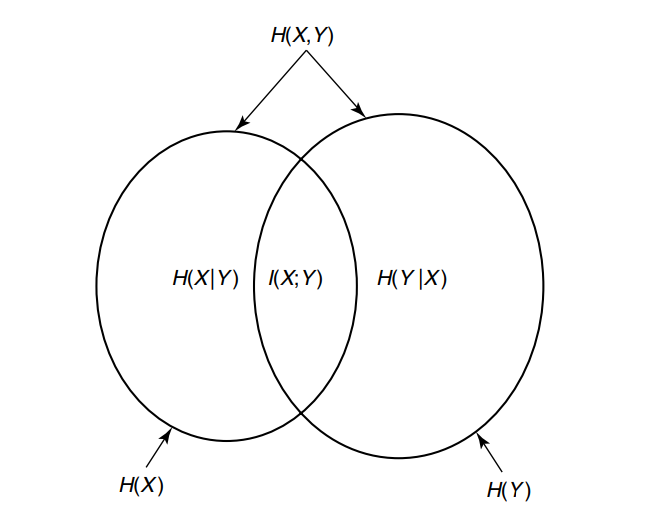
\includegraphics[width=8cm]{img/information_and_entropy.png}
    \caption{Relationship between entropy and mutual information.}
    \label{fig:information_and_entropy}
\end{figure}
Then from the theorem we have also that:
\begin{corollary}[Non negativity of mutual information]
    For any two random variables $X$ and $Y$,
    \begin{equation}
        I(X:Y) \geq 0
    \end{equation}
    with the equality holding iff $X$ and $Y$ are independent. 
\end{corollary}
Another useful result is
\begin{theorem}
    \begin{equation}
        h(X) \leq \log |\alp| \, ,
    \end{equation}
    with the equality holding iff $X$ is uniformly distributed.
\end{theorem}
\begin{proof}
    if $X$ is distributed w.r.t. $\mu$ and if $p(x)= \frac{1}{|\alp|}$ is the uniform distribution,
    \begin{equation*}
        o \leq d(\mu || p) = \sum_{x \in \alp} \mu(x) \log \frac{\mu(x)}{p(x)} = \log |\alp| - h(X) \, .
    \end{equation*}
\end{proof}
And finally from the positivity condition $0 \leq I(X:Y) = h(X) - h(X|Y)$ we have that
\begin{theorem}[Information can't hurt]
    \begin{equation}
        h(X|Y) \leq h(X)
    \end{equation}
    with equality holding iff $X$ and $Y$ are independent.
\end{theorem}
Intuitively, the theorem says that knowing another random variable $Y$ can only reduce the uncertainty in $X$. Note that this is true only on the
average. Specifically, $H (X|Y = y)$ may be greater than or less than or equal to $H (X)$, but on the average $H (X|Y ) =\sum_y p(y)H (X|Y = y) \leq H (X)$. For example, in a court case, specific new evidence might increase uncertainty, but on the average evidence decreases uncertainty.
\\Let's now end this chapter with some last properties of entropy. These come straightforward from the so called \textit{log sum inequality}:
\begin{theorem}[Log sum inequality]
    \begin{equation}
            \sum_{k=1}^n a_k \log \frac{a_k}{b_k} \geq \big( \sum_{k=1}^n a_k \big) \log \frac{\sum_{k=1}^n a_k}{\sum_{k=1}^n b_k}   
    \end{equation}
    with equality holding if and only if $\frac{a_k}{b_k}$ is constant. 
\end{theorem}
There are two consequences of the log sum inequality:
\begin{theorem}
\hfill
    \begin{itemize}
        \item[1)] Convexity of relative entropy:
        \\$d(\mu || \nu)$ is convex in the pair $(\mu, \nu)$, i.e. for any two pairs $(\mu_1, \nu_1)$ and $(\mu_2, \nu_2)$  and $\forall 0 \leq \lambda \leq 1$ we have 
        \begin{equation*}
            d(\lambda \mu_1 + (1 - \lambda) \mu_2 || \lambda \nu_1 + (1 - \lambda) \nu_2 ) \leq \lambda d (\mu_1 || \nu_1) + (1 - \lambda) d (\mu_2 || \nu_2)
        \end{equation*}
        \item[2)] Concavity of entropy:
        \\$h(\mu)$ is a concave function of $\mu$
    \end{itemize}
\end{theorem}
\begin{proof}
    \hfill
    Just apply the log sum inequality y to a single term of the left hand side and then sum over $x \in \alp$:
    \begin{equation*}
        \lambda \mu_1(x) \log \frac{\lambda \mu_1 (x)}{\lambda \nu_1 (x)} + (1 - \lambda) \mu_2(x) \log \frac{(1 - \lambda) \mu_2(x)}{(1 - \lambda) \nu_2(x)}
    \end{equation*}
    Concavity of entropy  follows from the convexity of the relative entropy $d$ and from the relation
    \begin{equation*}
        h(\mu) = \log |\alp| - d (\mu || p) \, ,
    \end{equation*}
    where $p(x)$ denotes the uniform probability distribution.
\end{proof}







\chapter{Ergodic Theorem, AEP Theorem and Entropy Theorem}
In this chapter we want to discuss the most important theorems of Information Theory: the \textit{Ergodic theorem}, the \textit{Asymptotic Equipartition Property (AEP) theorem} and the \textit{Shannon-McMillan-Breiman theorem} or \textit{Entropy theorem}.
\\First we will need to recall some concepts in probability convergence and state some fundamental results.

\section{Some fundamental results}
We say that a sequence of random variables $x_1, x_2, \dots, $ converges to a random variable $x$:
\begin{itemize}
    \item[a)] \textbf{in probability} if $\mathbb{P}(|x_n - x| > 0) \rightarrow 0$ when $n \rightarrow \infty$ and for all $\epsilon >0$
    \item[b)] \textbf{in mean square} if $\mathbb{E}( (x_n - x)^2 ) \rightarrow 0$ when $n \rightarrow \infty$
    \item[c)] \textbf{almost surely} (also called \textbf{with probability $\bm{1}$}) if 
    \begin{equation}
        \mathbb{P} \big( \lim_{n \rightarrow \infty} x_n = x \big) = 1
    \end{equation}
\end{itemize}
Of course $c) \Rightarrow b) \Rightarrow a)$. \\
If $\{P_n\}$ is a sequence of measurable properties (for example: $\frac{\sum_i^n x_i}{n} - \Bar{x}$ smaller or bigger than $\epsilon$) then
\begin{itemize}
    \item[1)] $P_n(x)$ holds \textbf{eventually almost surely}, if for almost every $x$ there is an $N=N(x)$ such that $P_n(x)$ is true for every $n \geq N$
    \item[2)] $P_n(x)$ holds \textbf{infinitely often}, almost surely, if for almost every $x$ there is an increasing sequence $\{n_j \}$ of integers (which may depend on $x$) such that $P_{n_j}(x)$ is true for $j = 1,2, \dots$
\end{itemize}
Here, $1) \Rightarrow 2)$. We also have three equivalent formulations of almost sure convergence:
\begin{lemma}
    The following are equivalent for measurable functions on a probability space:
    \begin{itemize}
        \item[1:] $f_n \rightarrow f$, almost surely;
        \item[2:] $|f_n(x) - f(x)| < \epsilon$, eventually almost surely, for every $\epsilon>0$;
        \item[3:] Given $\epsilon>0$, there is an $N$ and a set $G$ of measure at least $1 - \epsilon$ such that $|f_n(x) - f(x)| < \epsilon$, $x \in G$, $n \geq N$.
    \end{itemize}
\end{lemma}
\begin{lemma}[The Markov inequality]
\label{lemma:markov_ineq}
    Let $f$ be a nonnegative, integrable function on a probability space $(X, \Sigma, \mu)$. 
    \\If 
    \begin{equation*}
        \int f \, d \mu \leq \epsilon \delta
    \end{equation*}
    then 
    \begin{equation*}
        f(x) \leq \epsilon
    \end{equation*}
    except for a set of measure at most $\delta$. 
\end{lemma}
Next, we state a very deep and important result, the Borel-Cantelli principle \cite{Borel_cantelli}: such Lemma states that, under certain conditions, an event will have probability of either zero or one. Accordingly, it is the best-known of a class of similar theorems, known as zero-one laws.
\begin{lemma}[The Borel-Cantelli principle]
\label{lemma:borel_cantelly}
    If $\{E_n \}$ is s a sequence of measurable sets (so, a series of events) in a probability space $(X, \Sigma, \mu)$ such that
    \begin{equation*}
        \sum_n^{\infty} \mu(E_n) < \infty
    \end{equation*}
    then 
    \begin{equation*}
        x \notin E_n 
    \end{equation*}
    eventually almost surely, or equivalently 
    \begin{equation*}
        \mu \big( \limsup_{n \rightarrow \infty} E_n    \big) = 0
    \end{equation*}
\end{lemma}
Here, ``lim sup" denotes limit supremum of the sequence of events, and each event is a set of outcomes. That is, $\limsup E_n$ is the set of outcomes that occur infinitely many times within the infinite sequence of events $\{ E_n \}$. Explicitly,
\begin{equation*}
    \limsup_{n \rightarrow \infty} E_n = \cap_{n=1}^\infty \cup_{k=n}^\infty E_k
\end{equation*}
The set $\limsup E_n$ is sometimes denoted $\{E_n \, \text{i.o.} \}$, where ``i.o." stands for ``infinitely often". The theorem therefore asserts that if the sum of the probabilities of the events $E_n$ is finite, then the set of all outcomes that are ``repeated" infinitely many times must occur with probability zero. Note that no assumption of independence is required.
\\This basically means that such $E_n$ are becoming smaller and smaller with increasing $n$: thus if for example the sets $E_n$ are ``bad'' sets in which we do not want our variable $x$ to be, we just need to prove that $\sum_n \mu(E_n) < \infty$ to ``neglect them'' in the long run. 
\\A related result, sometimes called the \textbf{second Borel–Cantelli lemma}, is a partial converse of the first Borel–Cantelli lemma. The lemma states: If the events $E_n$ are (pairwise) independent and the sum of the probabilities of the $E_n$ diverges to infinity, then the probability that infinitely many of them occur is $1$. That is:
\begin{lemma}[second Borel–Cantelli lemma]
    if $\sum_{n=1}^\infty \mu(E_n) = \infty$ and the events $\{ E_n \}_{n=1}^\infty$ are \textbf{pairwise independent}, then 
    \begin{equation*}
        \mu \big( \limsup_{n \rightarrow \infty} E_n \big) = 1
    \end{equation*}
\end{lemma}
The infinite monkey theorem, that monkeys endless typing at random will, with probability $1$, eventually produce every finite text (such as the works of Shakespeare) \footnote{However, the probability that monkeys filling the entire observable universe would type a single complete work, such as Shakespeare's Hamlet, is so tiny that the chance of it occurring during a period of time hundreds of thousands of orders of magnitude longer than the age of the universe is extremely low (but technically not zero). To put it another way, for a one in a trillion chance of success of the monkeys typing Hamlet, there would need to be $10^{360641}$ observable universes where \textit{each proton} was a monkey typing.}, amounts to the statement that a (not necessarily fair) coin tossed infinitely often will eventually come up Heads. This is a special case of the second Lemma.
\\To end this section, we state an important result connecting cardinality and probability:
\begin{lemma}[cardinality bounds]
    Let $\mu$ be a probability measure on the finite set $A$, let $B \subset A$, and let $\alpha$ be a positive number.
    \begin{itemize}
        \item[1)] if $a \in B \Rightarrow \mu(a) \geq \alpha$, then $|B| \leq 1/\alpha$.
        \item[2)] For $b \in B$, $\mu(b) \geq \alpha/|B|$, except for a subset of $B$ of measure at most $\alpha$
    \end{itemize}
\end{lemma}
Basically, we are saying that given a set in a measurable space, this is \textbf{either big in probability or in cardinality}. We cannot have both. 

\section{AEP property and SMB Theorem}
In information theory, the analog of the law of large numbers is the asymptotic equipartition property (AEP). It is a direct consequence of the weak law of large numbers.
\begin{theorem}[AEP Theorem]
    \hfill \\
    If $x_1, x_2, x_3, \dots$ are i.i.d. which follow a distribution $p(x)$, then 
    \begin{equation}
        -\frac{1}{n} \log p(x_1, x_2, \dots, x_n) \xrightarrow{\text{in probability}}  H(x)
    \end{equation}
\end{theorem}
\begin{proof}
\hfill
\\
    Functions of independent random variables are also independent random variables. Thus, since the $x_i$ are i.i.d., so are $\log p(x_i)$. Hence, by the weak law of large numbers, 
    \begin{equation*}
        -\frac{1}{n} \log p(x_1, x_2, \dots, x_n) = -\frac{1}{n} \sum_i \log p(x_i) \xrightarrow{\text{in probability}} - \mathbb{E}[\log p(x)] = H(x)
    \end{equation*}
    which proves the theorem.
\end{proof}
We can also give an alternative (and equivalent) formulation of the AEP Theorem, stated under the assumptions of considering a  discrete-time stationary ergodic process $\mu$: the asymptotic equipartition property for such stochastic source is known as the Shannon–McMillan–Breiman theorem (SMB).
\begin{theorem}[SMB Theorem]
\label{th:SMB}
    \hfill \\
    Consider a stationary, ergodic, stochastic source $\mu$ with entropy $h = h_\mu > 0$. For simplicity, here we also assume that we are dealing with an i.i.d. process (but the more general case is also true).
    \\Then for every $\epsilon>0$ and all sufficiently large $n$, one can find a subset $\mathcal{T}_n \subset \alp^n$ of \textbf{typical sequences} that is \textbf{small} in cardinality, but \textbf{large} in probability, so that:
    \begin{itemize}
        \item[(1)] $e^{n (h- \epsilon)} \leq |\mathcal{T}_n| \leq e^{n (h+ \epsilon)}$
        \item[(2)] $\lim_{n \rightarrow \infty} \mu(\mathcal{T}_n) = 1$
        \item[(3)] For each $\omega \in \mathcal{T}_n$ we have
        \begin{equation*}
            e^{n (h- \epsilon)} \leq \mu(\omega) \leq e^{n (h+ \epsilon)}
        \end{equation*}
    \end{itemize}
\end{theorem}
Let's take a closer look at what this theorem is telling us.
\\If we consider $|\alp|=m$, then $|\alp^n| = m^n = e^{n \log m}$. Also, we know from the basic properties of entropy that $0 \leq h \leq \log n$. If we then look at the ratio $\frac{|\mathcal{T}_n|}{|\alp^n|} \sim e^{-n (\log m - h)} \xrightarrow[n \rightarrow \infty]{} 0$. This is what we mean by ``small'' in cardinality: not in a general sense, but small with regard to the dimension of our alphabet. 
\\Also, we are saying that $\mu(\mathcal{T}_n) \rightarrow 1$ as $n \rightarrow \infty$: i.e., the ``density'' of $\mathcal{T}_n$ in $\alp^n$ is becoming bigger and bigger as we increase $n$. In the limit of $n$ going to infinity, the measure of our typical set becomes $1$: hence, in such limit \textbf{all sequences are typical}. 
\\All of this is just to say that under suitable conditions, we will always have in our alphabet a few sequences with are typical with respect to all of those which can be formed: think as always about words in a language versus all the combinations of letters that can be formed. 
\\Also, the last statement is telling us that $\mu(\omega) \sim e^{-n h}$, which is up to an $\epsilon$ equivalent to saying that $\lim_{n \rightarrow \infty} \frac{1}{n} \log \mu(\omega_n) = h$ as in the first formulation.
\begin{proof}
    \hfill \\ 
    Given $\epsilon>0$, we let $\delta=\delta(\epsilon)$ to be chosen later.
    \\We select  finite sequences with good empirical distribution:
    \begin{equation*}
        \mathcal{T}_n \equiv \{ \omega \in \alp^n : \big| \frac{f_\omega(a_k)}{n} - \mu_k \big| \leq \delta, \, k=1,2,\dots, d \}
    \end{equation*}
    The second statement follows immediately from the Law of Large Numbers: $\lim_{n \rightarrow \infty} \mu(\mathcal{T}_n) = 1$.
    \\In the i.i.d. case we are discussing here:
    \begin{align*}
        \mu(\omega) = & \prod_{j=1}^n \mu(\omega_j) = \prod_{k=1}^d \mu_k^{f_\omega(a_k)} =  \\
        = & \exp \big( \sum_{k=1}^d f_\omega(a_k) \ln \mu_k \big) = \exp \big( n \sum_{k=1}^d \frac{f_\omega(a_k)}{n} \ln \mu_k \big) = & \\
        = & \exp \big( n \sum_{k=1}^d \mu_k \ln \mu_k \big) \cdot \exp \big( n \sum_{k=1}^d (\frac{f_\omega(a_k)}{n} - \mu_k) \ln \mu_k \big) = & \\
        = & \exp \bigg( n (-h + \sum_{k=1}^d (\frac{f_\omega(a_k)}{n} - \mu_k) \ln \mu_k) \bigg)
    \end{align*}
    Now we choose $\delta$ sufficiently small such that $\big|  \sum_{k=1}^d (\frac{f_\omega(a_k)}{n} - \mu_k) \ln \mu_k) \big| \leq \epsilon$, for $\omega \in \alp^n$, and this gives the first statement of the Theorem.
    \\Furthermore, 
    \begin{equation*}
        1 \geq \mu(\mathcal{T}_n) = \sum_{\omega \in \alp^n} \mu(\omega) \geq e^{-n (h + \epsilon)} |\mathcal{T}_n|
    \end{equation*}
    i.e., $|\mathcal{T}_n| \leq e^{n(h+ \epsilon)}$.
    \\On the other hand, for sufficiently large $n$ we will have that
    \begin{equation*}
        \frac{1}{2} \leq \mu(\mathcal{T}_n) \leq e^{-n(h - \frac{\epsilon}{2})} |\mathcal{T}_n| \, ,
    \end{equation*}
    i.e., for sufficiently large $n$
    \begin{equation*}
        |\mathcal{T}_n| \geq \frac{1}{2} e^{n(h - \frac{\epsilon}{2})} \geq e^{n(h - \epsilon)} 
    \end{equation*}
    and this gives the first statement.
\end{proof}
We now want to prove a a result much stronger than the SMB theorem: the \textbf{Entropy Theorem}

\section{Entropy Theorem and Ergodic Theorem}

\begin{theorem}[Entropy Theorem]
\label{th:entropy_theorem}
\hfill \\
    Given a stochastic,stationary, ergodic process $\mu$ on $\alp$,
    \begin{equation}
        \lim_{n \rightarrow \infty} -\frac{1}{n} \log \mu(x_1^n) = h_\mu \qquad \text{\textbf{almost surely}}
    \end{equation}
\end{theorem}
We want to prove this by introducing and using a beautiful technique
developed by Ornstein and Weiss while they were trying to extend entropy theorem
from stochastic processes to random fields. In order to introduce the first fundamental lemmas concerning packings and covering, It is useful to start by proving the Ergodic Theorem.
\\Recalling that a process $\mu$ is ergodic if any shift-invariant subset is either of measure $1$ or $0$, we state and prove the ergodic theorem in its essential form assuming (without loss of generality) a binary process $\alp= \{0,1 \}$
\begin{theorem}[Ergodic Theorem]
\hfill \\
    If $\mu$ is a (binary) stationary, ergodic process
    \begin{equation*}
        \lim_{n \rightarrow \infty} \frac{1}{n} \sum_{j=1}^n x_j \quad \text{exists \textbf{almost surely} on } \alp^{\nb}
    \end{equation*}
\end{theorem}
In this case, letting $p = \mathbb{E}(x_1) = \mu(x_1=1)$, the theorem asserts that 
\begin{equation*}
    \lim_{n \rightarrow \infty} \frac{1}{n} (x_1 + x_2 +\dots+ x_n) = p \qquad \text{almost surely}
\end{equation*}
\begin{proof}
    We start by assuming that the Theorem is false: the superior (inferior) limit of the averages is then larger (smaller) than $p$ by a fixed amount on a set of positive measure.
    \\By assumption there exists $\epsilon>0$ such that if 
    \begin{equation*}
        A_\epsilon \equiv \big\{ x \in \alp^n : \limsup_{n \rightarrow \infty} \frac{x_1 + x_2 +\dots+ x_n}{n} > p + \epsilon \big\}
    \end{equation*}
    then $\mu(A_\epsilon) > 0$.
    \\It is then easy to see (\textit{exercise - and an important one}) that $A_\epsilon$ is \textit{invariant}, hence of measure one: 
    \begin{equation*}
        \mu(A_\epsilon) = 1
    \end{equation*}
    This means that for almost all sequences $x$, there exists an infinite partition ($x$-dependent) in disjoint intervals over which the average exceeds $p+\epsilon$.
    \\i.e. given $x= x_1, x_2, \dots $ and $n \in \nb^+$, we denote by $m=m(n) > n$ the first time
    for which the average over the interval $[n, m]$ exceeds the expected value $p$ by $\epsilon$. 
    \\$m$ is also $x$ dependent, and it is also finite for all $n$ and for a set of full measure of $x$'s in $\alp^{\nb}$.
    \\It follows that for almost all $x$, we can find a disjoint partition ($x$ dependent):
    \begin{equation*}
        \nb = \cup_{k=1}^\infty [n_k, m_k], \quad \text{with} \, \, m_0 = 0, \, n_k = m_{k-1}+1
    \end{equation*}
    and 
    \begin{equation*}
        \frac{1}{m_k - n_k + 1} \sum_{j=n_k}^{m_k} x_j > p + \epsilon \, .
    \end{equation*}
    The important step is now to obtain a control over finite sequences, proving that for sufficiently large $N$ there exists a set $\mathcal{G}_N$, large in probability, on which the average beats $p+\epsilon$.
    Let's formally state this last passage: 
    \begin{lemma}
    \label{lemma:ergodic_th}
        Given $\delta>0$ there exists a positive integer $N$ and a set $\mathcal{G}_N \subset \alp^N$ such that
        \begin{itemize}
            \item[1)] $\mu(\mathcal{G}_N)> 1 - \delta$
            \item[2)] For each $\omega_1^n = (\omega_1, \dots, \omega_n) \in \alp^N$ there are disjoint intervals $[n_i, m_i] \subset [1,N]$ such that 
            \begin{itemize}
                \item[a)] $\{ [n_i,m_i] \}$ is a $\delta-$cover of $[1,N]$, i.e. $\sum_i (m_i - n_i +1) > (1 - \delta)N$
                \item[b)] On each element of the coverings, the average exceeds $p$:
                \begin{equation*}
                    \frac{1}{|\omega_{n_i}^{m_i}|} \sum_{j=n_i}^{m_i} \omega_j > p + \epsilon
                \end{equation*}
            \end{itemize}
        \end{itemize}
    \end{lemma}
    This basic lemma leads to our desired contradiction.
    \\As a matter of fact, if $\omega_1^n \in \mathcal{G}_N$ then 
    \begin{equation*}
        \sum_{j=1}^N \omega_j \geq \sum_i \sum_{j=n_i}^{m_i} \omega_j \geq (1 - \delta) N (p + \epsilon)
    \end{equation*}
    hence
    \begin{equation*}
        p = \mathbb{E} \bigg[ \frac{1}{N} \sum_{j=1}^N X_j \bigg] \geq (1 - \delta) (p + \epsilon) \mu(\mathcal{G}_N) \geq (1 - \delta)^2 (p+\epsilon)
    \end{equation*}
    which can not be true for all $\delta$.
\end{proof}
Let's now see for completeness the proof of the Lemma:
\begin{proof}[proof of Lemma \ref{lemma:ergodic_th}]
    The first observation is that the lengths $L_n = ( m(n) -n +1 )$ of the intervals where the average is larger then $p + \epsilon$ is in fact bounded, except for a set of (arbitrary) small probability.
    \\Namely, there exists an $L$ such that $\mu(L_n > L) < \delta^2/2$.
    \\We now define $c_n$ to be $1$ if $L_n>L$ and $0$ otherwise, so that, for any $N$,
    \begin{equation*}
        \mathbb{E} \bigg[ \frac{1}{N} \sum_{n=1}^N c_n \bigg] < \frac{\delta^2}{2}
    \end{equation*}
    The Markov inequality (\ref{lemma:markov_ineq}) yields:
    \begin{equation*}
        \mu \bigg( \frac{1}{N} \sum_{n=1}^N c_n < \frac{\delta^2}{2} \bigg) > 1 - \delta
    \end{equation*}
    For $N>L$ we define $\mathcal{G}_N$ to be the event
    \begin{equation*}
        \frac{1}{N-L+1} \sum_{n=1}^{N-L+1} c_n < \frac{\delta}{2}.
    \end{equation*}
    The Markov inequality gives the first property of the basic Lemma.
    \\For each $(\omega_1, \dots, \omega_N) \in \mathcal{G}_N$ we define the intervals $[n_j, m_j]$ inductively, putting 
    \begin{equation*}
        n_1 = \min \{ n \geq 1: L_n \leq L \}, \quad m_1 = m(n_1)
    \end{equation*}
    and 
    \begin{equation*}
        n_{j+1} = \min \{ n > m_j : L_n \leq L \}, \quad m_{j+1} = m(n_{j+1}).
    \end{equation*}
    i.e.,  we go from a covering to a packing with gaps. The construction stops the first time $m_j$ exceeds $N-L+1$.
    \\The first of the second properties of the Basic Lemma is now true by definition of $n_j$ and $m_j$.
    \\An integer $n$ in $[1,N]$  fails to be in one of the intervals $[n_j, m_j]$ only if $L_n > L$ or if $n > N - L + 1$.
    \\By definition of $\mathcal{G}_N$ there are at most $N\delta/2$ indices $n$ in $[1,N]$ for which $L_n > L$.
    \\Furthermore if we choose $N \geq 2L/\delta$ then $N-L+1, N$ contains at most $N\delta/2$ integers.
\end{proof}

\section{From coverings to packings}
Now we want to discuss four Lemmas\footnote{From now on, this is \textbf{additional and optional material}} : the packing Lemma, the counting
Lemma, the doubling Lemma and the strong doubling Lemma; the first two are strictly combinatorial, while the second two are just extensions of the Ergodic Theorem.
\\The word doubling come from the fact that the applications of these
lemmas rely on the success on some other limit theorem, a
convergence-in-probability theorem for doubling and an almost-sure theorem for strong doubling. 
\\At the end we will then introduce, discuss and prove the so called strong packing lemma that will be used in the proof of the optimality of the Lempel-Ziv code.

\subsection{Packing and counting}
The packing technique is a method for building ``almost'' packings of intervals from ``almost" covering by subintervals whose left end points already cover most of the interval. 
\\In more mathematical terms: 
\begin{definition}
    \hfill
    \\Given an interval of integers $[1, N]$ and a collection $\mathcal{C}$ of distinct subintervals, $\mathcal{C}= \{ n_j, m_j \}$ with $1 \leq n_j \leq m_j \leq N$, we say that
    \begin{itemize}
        \item[(1)] $\mathcal{C}$ is called a \textbf{strong} $\bm{1 - \delta}$- \textbf{cover} of $[1, N]$ if the left points cover at least a $1- \delta$ fraction of $[1, N]$:
        \begin{equation*}
            |\{ n_j : [n_j, m_j] \in \mathcal{C} \}| > (1 - \delta)N \,.
        \end{equation*}
        \item[(2)] $\mathcal{C}$ is called a $\bm{1 - \delta}$- \textbf{packing} if it is \textbf{disjoint} and its union cover at least $(1 - \delta)$-fraction of $[1,N]$:
        \begin{equation*}
            \sum_{[n_j, m_j] \in \mathcal{C}} |(m_j - n_j + 1)| \geq (1 - \delta)N \, .
        \end{equation*}
        \item[(3)] $\mathcal{C}$ is $\bm{L-}$ \textbf{bounded}  if $|(m_j - n_j +1 )| \leq L$, for each $[n_j, m_j] \in \mathcal{C}$
    \end{itemize}
\end{definition}
\begin{lemma}[The packing lemma]
\hfill\\
    if $N \geq L/\delta$, then any $L-$bounded, strong $1-\delta$ cover $\mathcal{C}$ of $[1,N]$ contains a $(1- 2\delta)-$packing.
\end{lemma}
The next counting lemma gives us bounds on the number of sequences that are mostly packed by block drawn from fixed collections whose size are known, which we usually consider to be the collections of typical sequences provided by the AEP theorem, or similar.
\\First we need few notations: let $\delta$ and $M$ be positive numbers: for each $m \geq M$, we have subsets $\mathcal{B}_m \subset \alp^m$ and we denote 
\begin{equation*}
    \mathcal{B}_M = \cup_{m \geq M} \mathcal{B}_m
\end{equation*}
Then we define:
\begin{definition}
    A sequence $x_1^N \in \alp^N$ is said to be $(1- \delta)-$built-up from $\mathcal{B}$ if it can be parsed in variable length blocks as 
    \begin{equation}
        x_1^N= b_1b_2\dots b_k, \quad \text{s.t.} \, \, \sum_{j: b_j \in \mathcal{B}} |b_j| \geq (1-\delta)N
    \end{equation}
\end{definition}
We denote by $G_N$ the subset of $\alp^N$ given by the sequences $x_1^N$ that are $(1-\delta)-$built-up from $\mathcal{B}_M$ .
\begin{lemma}[The Counting Lemma]
\hfill \\
    If $|\mathcal{B}_m| \geq 2^{m (h+\epsilon)}$, $h_b(2/M) \leq \epsilon/2$ and $\delta \log |\alp| \leq \epsilon/2$, then 
    \begin{equation*}
        |G_N| \leq 2^{N(h + 2\epsilon)}\, .
    \end{equation*}
\end{lemma}
where 
\begin{equation}
\label{eq:binary_entropy}
    h_b(p) = -p \log p - (1-p) \log(1-p)
\end{equation}
denotes the binary entropy function.
\begin{proof}
    \hfill \\
    We first condition on the locations of the blocks that belong to $\mathcal{B}_M$: a \textbf{skeleton} $\mathcal{P}= \{ [n_j, m_j] \}$ is a disjoint collection of subintervals such that
    \begin{itemize}
        \item[a)] $[n_j, m_j] \subset [1,N]$ and $ (m_j - n_j + 1) \geq M$;
        \item[b)] $\sum_{[n_j, m_j] \in \mathcal{P}} (m_j - n_j + 1) \geq (1 - \delta) N $  . 
    \end{itemize}
    We now say that $x_1^N \in G_N$ is compatible with the skeleton $\mathcal{P}$  if the word $x_i^j$ belongs to $\mathcal{B}_M$ whenever the interval $[i,j]$ belongs to $\mathcal{P}$, and we denote by $G_N(\mathcal{P}) \subset G_N$ the set of all the sequences compatible with the skeleton $\mathcal{P}$. \\
    Clearly,
    \begin{equation*}
        G_N \equiv \cup_{\mathcal{P}} G_N (\mathcal{P}) \, .
    \end{equation*}
    It is now easy to see that:
    \begin{equation*}
        |G_N (\mathcal{P})| \leq 2^{N (h+\epsilon)} |\alp|^{\delta N} \, .
    \end{equation*}
    The first term $2^{N (h+\epsilon)}$ come from the fact that any subinterval $[i, j]$ of length $m$ can be filled in at most $2^{m (h+\epsilon)} \geq |\mathcal{B}_M|$ ways, whereas there are at most $|\alp|^{\delta N}$ ways to fill the places that do not belong to $\mathcal{P}$.\\
    Each interval in a skeleton has length at least $M$, so at most $2N/M$ points can be endpoints of its intervals. Thus the number of possible skeletons is upper bounded by
    \begin{equation*}
        \sum_{j \leq 2N/M} 
        \begin{pmatrix}
            N \\
            j
        \end{pmatrix}
        \leq 2^{N h_b (2/M)}
    \end{equation*}
    The set $G_N$ is the union of the sets $G_N(\mathcal{P})$ over all skeletons $\mathcal{P}$, so the cardinality of $G_N$ is upper bounded by the product of the two previous bounds, that is
    \begin{equation*}
        \log |G_N| \leq N (h + \epsilon) + \delta N \log |\alp| + N h_b (2/M) \, .
    \end{equation*}
    This is bounded by $N (h + 2\epsilon)$ if $h_b (2/M) \leq \epsilon/2$ and $\delta \log |\alp|$ .
\end{proof}

\subsection{Doubling}
We now want to prove that in certain situations, given sequences of blocks $\mathcal{B}_n \subset \alp^n$ provided by some convergence in probability limit theorem, eventually almost surely, most indices in $x_1^N$ are in fact starting points of blocks from the $\mathcal{B}_n$'s.
\begin{lemma}[Doubling Lemma]
    \hfill \\
    If $\mu(\mathcal{B}_n) > 1 - \delta/2$ then, eventually almost surely as $N \rightarrow \infty$
    \begin{equation*}
        x_j^{j+n-1} \in \mathcal{B}_n \quad \text{for at least $(1-\delta)N$ indices $j \in [1, N-n+1]$}
    \end{equation*}
\end{lemma}
\begin{proof}
    Given $x \in \alp^{\nb}$, the number of indices $j \in [1, N-n+1]$ for which $x_j^{j+n-1} \in \mathcal{B}_n$ is given by 
    \begin{equation*}
        \sum_{j=1}^{N-n+1} \chi_{U_n} (\sigma^{j-1} x)
    \end{equation*}
    where 
    \begin{equation*}
        U_n \equiv \{ x : x_1^k \in \mathcal{B}_k \}
    \end{equation*}
    By the ergodic theorem, almost surely,
    \begin{equation*}
        \lim_{n \rightarrow \infty} \frac{1}{N-n+1} \sum_{j=1}^{N-n+1} \chi_{U_n} (\sigma^{j-1} x) = \mu(U_n) = \mu(\mathcal{B}_n) > 1 - \frac{\delta}{2} \, .
    \end{equation*}
\end{proof}
In applications, often some almost sure limit Theorems provide a sequence of set $\mathcal{B}_n \in \alp^n$ such that $x_1^n \in \mathcal{B}_n$ eventually almost surely.
\\In this case we can prove that every block in $x_1^n$ that starts at $j$ and has length larger than $n$ belongs to $\cup_{i \geq n} \mathcal{B}_i$
\begin{lemma}[Strong-Doubling Lemma]
    \hfill \\
    If $x_1^n \in \mathcal{B}_n$, eventually almost surely as $n \rightarrow \infty$, then given $\delta>0$  there is an $N$ such that, eventually almost surely as $N \rightarrow \infty$, we have that
    \begin{equation*}
        x_j^{j+n-1} \in \mathcal{B}_n \, , \quad x_j^{j+n} \in \mathcal{B}_{n+1}, \dots, x_j^N \in \mathcal{B}_{N-j+1}
    \end{equation*}
    holds for $x_1^n$ for at least $(1 - \delta)N$ indices $j \in [1, N-n+1]$
\end{lemma}
\begin{proof}
    \hfill \\
    The assumption $x_1^n \in \mathcal{B}_n$, eventually almost surely, implies that for $n$ large enough $\mu(U_n) > 1 - \delta/4$, where
    \begin{equation*}
        U_n \equiv \{ x : x_1^j \in \mathcal{B}_j, \, \forall \, j \geq n \} \, .
    \end{equation*}
    Again from the Ergodic Theorem, 
    \begin{equation*}
        \lim_{n \rightarrow \infty} \frac{1}{N-n+1} \sum_{j=1}^{N-n+1} \chi_{U_n} (\sigma^{j-1} x) = \mu(U_n)
    \end{equation*}
    so that, in particular,
    \begin{equation}
    \label{eq:strong_doubling}
         \frac{1}{N-n+1} \sum_{j=1}^{N-n+1} \chi_{U_n} (\sigma^{j-1} x) \geq 1 - \frac{\delta}{2}, \quad \text{eventually almost surely as $N \rightarrow \infty$}
    \end{equation}
    Suppose \ref{eq:strong_doubling} holds for a given $N$.
    \\This means that $\sigma^{j-1} x \in U_n$ for at least $(1 - \delta/2)N$ indices $j \in [1, N - n+1]$, namely, all blocks in the infinite sequence $x$ that start at $j$ and have length at least $n$ must belongs to $\cup_{j \geq n} \mathcal{B}_j$.
    \\In particular, if $\sigma^{j-1} x \in U_n$ and $j \geq N-n$, then all blocks in the finite sequence $x_1^N$ that starts at $j$ and have length at least $n$ must belong to $\cup_{j \geq n} \mathcal{B}_j$. 
    \\If $N \geq 2n/\delta$ there will be at most $\delta N/2$ indices in the interval $[N-n+1,N]$.
    \\Thus, if \ref{eq:strong_doubling} holds and $N \geq 2n/\delta$, then for $x_1^N$ the strong doubling condition must
    hold for at least $(1 - \delta)N$ indices $j \in [1, N-n+1]$.
    \\This proves the lemma since \ref{eq:strong_doubling} holds eventually almost surely as $N \rightarrow \infty$.
\end{proof}
Now we can finally prove the Entropy Theorem:
\begin{proof} [proof of Th. \ref{th:entropy_theorem} (Entropy Theorem)]
\hfill \\
    Define $h(x) = \liminf_{n \rightarrow \infty} \log \mu(x_1^n)$.
    \\Since $h(\sigma x) \leq h(x)$ and because of ergodicity, $h(x) = h$ is constant almost surely. 
    \\We want to prove that also 
    \begin{equation*}
        h = \limsup_{n \rightarrow \infty} -\frac{1}{n} \log \mu(x_1^n) \, .
    \end{equation*}
    Fix $\epsilon > 0$; by the definition of $\liminf$ and taking the exponential:
    \begin{equation}
    \label{eq:proof_of_entropy_th}
        \mu(x_1^n) \geq 2^{-n (h+\epsilon)}, \quad \text{infinitely often, almost surely}.
    \end{equation}
    The main idea of the proof is to show that, eventually almost surely, as $N \rightarrow \infty$, most indices $j \in [1, N]$ are starting places of blocks in $x_1^N$ for which $\mu(x_j^{j+N-1}) \geq 2^{-n(h+\epsilon)}$ for some $n \leq N-j$.
    \\Then we will use the packing lemma to extract an almost packing and the counting lemma to show that the set of $N-$sequences that have such an almost packing cannot have cardinality exponentially much bigger than $2^{N(h+\epsilon)}$.
    \\Even if \ref{eq:proof_of_entropy_th} does not give us any control on $n$, starting at $j$, the waiting time $n$ until $\mu(x_j^{j+n-1}) \geq 2^{-n(h+\epsilon)}$ occurs is  almost surely finite, and therefore is bounded except for a set of small probability.
    
    Let $M$ so that $h_b(2/M) \leq \epsilon/2$ (again, $h_b$ represents binary entropy as in \ref{eq:binary_entropy} and we fix $\delta>0$ such that $\delta \log |\alp| \leq \epsilon/2$). 
    \\Let $L \ geq M$ be an integer to be specified later, and let $\mathcal{B}= \cup_{M \leq n \leq L} \mathcal{B}_n$ where
    \begin{equation*}
        \mathcal{B}_n = \{ x_1^n : \mu(x_1^n) \geq 2^{-n(h+\epsilon)}\} \subset \alp^n \, .
    \end{equation*}
    Finally, for $N \geq L$, we let 
    \begin{equation*}
        G_N \equiv \{ x_1^n \in \alp^N : x_1^n \, \text{is} \,\, (1-\delta)- \text{built up from $\mathcal{B}$}\} \, .
    \end{equation*}
    Since $|\mathcal{B}_n| \leq 2^{n(h+\epsilon)}$, the counting lemma implies that 
    \begin{equation*}
        |G_N| \leq 2^{N(h + 2\epsilon)} \, .
    \end{equation*}
    Then the following lemma (which we will prove later on)
    \begin{lemma}
    \label{lemma:proof_entropy_th}
        \hfill \\
        If $L$ is large enough, then $x_1^N \in G_N$, eventually almost surely.
    \end{lemma}
    implies that
    \begin{equation*}
        \mu(V_n) \leq |G_n| 2^{-n(h+3\epsilon)}
    \end{equation*}
    where 
    \begin{equation*}
        V_n \equiv \{ x_1^n \in G_n : \mu(x_1^n) \leq 2^{-n()h+3\epsilon} \}
    \end{equation*}
    Now because $\sum_n \mu(V_n) < \infty$, by the Borel-Cantelli principle (\ref{lemma:borel_cantelly}) $x_1^n \notin V_n$ eventually almost surely, which, since $x_1^n \in G_n$ eventually almost surely, implies that $\mu(x_1^n) \geq 2^{-n(h+3\epsilon)}$ eventually almost surely.
    \\This means that $h = \limsup_{n \rightarrow \infty} -\frac{1}{n} \log \mu(x_1^n)$, with probability $1$, and the Entropy Theorem is proved.
\end{proof}
We give now the proof of the Lemma \ref{lemma:proof_entropy_th}.
\begin{proof}[proof of \ref{lemma:proof_entropy_th}]
\hfill \\
    Let’s go back to the proof of the previous lemma: we must show how $L \geq M$ can be chosen so that $x_1^N \in G_N$ , eventually almost surely.
    \\The random variable $n(x)$, given by the least integer $n \geq M$ for which $x_1^n \in \mathcal{B}$ is almost surely finite.
    \\Thus we can choose $L \geq M$ such that $n(x) \leq L$, with probability at least $1 - \delta/4$.
    \\This means that the set 
    \begin{equation*}
        U_L = \{ x_1^L : x_1^j \\in \mathcal{B}_j, \, \text{for some $j \in [M, L]$} \}
    \end{equation*}
    has measure at least $1 - \delta/4$
    \\Applying the doubling lemma to the set $U_L \subseteq \alp^L$ we get that for $x_1^N$ eventually almost surely as $N \rightarrow \infty$ there will be at least $(1 - \delta/2)N$ indices $j \in [1, N-L+1]$ for which $x_j^{j+L-1} \in U_L$.
    \\Then the collection $\{ [i,j] : x_i^j \in \mathcal{B} \}$ is an $L-$bounded, strong $(1- \delta/2)-$cover of $[1,N]$, so that once $N$ is large enough to satisfy $N \geq 2L/\delta$, the packing lemma implies that $x_1^N$ is $(1 -\delta)-$built up from $\mathcal{B}$, that is, $x_1^N \in G_N$.
    \\This proves the lemma and completes the proof of the Entropy Theorem.
\end{proof}

\subsection{Strong-packing}
We need to strength further the packing results in order to be able to prove the optimality of the \textit{Lempel-Ziv codes}.
\begin{definition}[word and parsing]
\hfill \\
    A finite sequence $\omega$ is called a word of length $|\omega|$ (we already introduced this) and a \textbf{parsing} of $x_1^n$ is an ordered collection $\mathcal{P} = \{ \omega(1), \omega(2), \cdots, \omega(t) \}$ of words for which 
    \begin{equation*}
        x_1^n = \omega(1) \omega(2) \cdots \omega(t)
    \end{equation*}
\end{definition}
\begin{definition}[Strong-Packing]
\hfill\\
    Fix a sequence of sets $\{\mathcal{T}_k \}$, such that $\mathcal{T}_k \subseteq \alp^k$, for $k \geq 1$. 
    \\A parsing $x_1^n = \omega(1) \omega(2) \cdots \omega(t)$ is $(1 - \epsilon)-$built up from $\{\mathcal{T}_k \}$, or $(1 - \epsilon)-$packed by $\{\mathcal{T}_k \}$, if the words that belong to $\cup \mathcal{T}_k$ cover at least $(1 - \epsilon)-$fraction of $n$, i.e.
    \begin{equation*}
        \sum_{\omega(j) \in \cup \mathcal{T}_k} |\omega(j)| \geq (1 - \epsilon) n \, .
    \end{equation*}
    A sequence $x_1^n$ is $(K, \epsilon)-$strongly-packed by $\{\mathcal{T}_k \}$ if \textbf{any} parsing $x_1^n = \omega(1) \omega(2) \cdots \omega(t)$ for which 
    \begin{equation*}
        \sum_{|\omega_j| < K} |\omega_j| \leq \frac{\epsilon n}{2} \, ,
    \end{equation*}
    is $(1 - \epsilon)-$built-up from $\{\mathcal{T}_k \}$.
\end{definition}
Strong-packing captures the essence of the idea that if the long words of a parsing cover most of the sample path, those long words that come from fixed collections  $\{\mathcal{T}_k \}$ must cover most of the sample path.
\\The key result is the existence of collections for which the $\mathcal{T}_k$’s are of exponential size determined by entropy and such that eventually almost
surely $x_1^n$ is almost strongly-packed.
\begin{lemma}[Strong-packing lemma]
    Let $\mu$ be an ergodic process of entropy $h=h_\mu$ and let $\epsilon$ be a positive number.
    \\There is an integer $K=K(\epsilon)$ and, for each $k\geq K$, a set $\mathcal{T}_k = \mathcal{T}_k(\epsilon) \subseteq \alp^k$, such that both of the following hold:
    \begin{itemize}
        \item[(1)] $|\mathcal{T}_k| \leq 2^{k(h+ \epsilon)}$ for $k \geq K$;
        \item[(2)] $x_1^n$ is eventually almost surely $(K, \epsilon)-$strongly-packed by $\{\mathcal{T}_k \}$.
    \end{itemize}
\end{lemma}
The proof is a little bit complex but the idea behind it is kind of simple.
\\The entropy theorem provides an integer $m$ and a set $C_m \subseteq \alp^m$ of measure close to $1$ and cardinality at most $2^{m(h+ \delta)}$.
\\By the Ergodic Theorem, eventually almost surely most indices in $x_1^n$ are starting places of $m-$blocks from $C_m$.
\\But if such an $x_1^n$ is partitioned into words, then by the Markov inequality (\ref{lemma:markov_ineq}) most of $x_1^n$ must be covered by those words whihc themselves have the property that most of their indices are starting places of members of $C_m$.
\\If a word is long enough, however, and most of its indices are starting places of members of $C_m$, then the word is mostly built-up from $C_m$, by the packing lemma.
\\The collection $\mathcal{T}_k \subseteq \alp^k$ of words that are mostly built up from $C_m$ has cardinality only a small exponential factor more than $2^{k(h+\delta)}$ (by the built-up set lemma).
\\Let's be more rigorous:
\begin{proof}
    Fix $\epsilon>0$, and let $\delta>0$ to be specified later on.
    \\The entropy theorem provides an $m$ for which the set 
    \begin{equation*}
        C_m \equiv \{ a_1^m  : \mu(a_1^m) \geq 2^{-m(h+\delta)}\}
    \end{equation*}
    has measure at least $1-\delta^2/4$.
    \\For $k \geq m$, let $\mathcal{T}_k$ be the set of sequences of length $k$ that are $(1-\delta)-$built-up from $C_m$.
    By the built-up set lemma, it can be supposed that $\delta$ is small enough to guarantee that 
    \begin{equation*}
        |\mathcal{T}_k| \leq 2^{k(h+\epsilon)}, \quad k \geq m \, .
    \end{equation*}
    By making $\delta$ smaller, if necessary, it can be supposed that $\delta < \epsilon/2$.
    \\It remains to show that eventually almost surely $_1^n$ is $(K, \epsilon)-$strongly-packed by $\{ \mathcal{T}_k\}$, for suitable $K$.
    \\This is a consequence of the following three observations
    \begin{itemize}
        \item[1)] The ergodic theorem implies that for almost every $x$ there is an $N=N(x)$ such that for  $n \geq N$ the sequence $x_1^n$ has the property that $x_j^{j+m-1} \in C_m$ for at least $(1 - \delta^2/2)n$ indices $j \in [1, n-m+1]$, i.e., $x_1^n$ is $(1 - \delta^2/2)-$strongly-covered by $C_m$.
        \item[2)] If $x_1^n$ is $(1 - \delta^2/2)-$strongly-covered by $C_m$ and parsed as $x_1^n = \omega(1) \omega(2) \cdots \omega(t)$, then by the Markov inequality, the words $\omega(j)$ that are not $(1 - \delta/2)-$strongly-covered by $C_m$ cannot have total length more than $\delta n \leq \epsilon n /2$.
        \item[3)] If $\omega(j)$ is $(1 - \delta/2)-$strongly-covered by $C_m$, and if $|\omega(j)| \geq 2/\delta$, then by the packing lemma $\omega(j)$ is $(1 - \delta)-$packed by $C_m$, that is, $\omega(j) \in \mathcal{T}_{|\omega(j)|}$.
    \end{itemize}
    From the preceding it is enough to take $K\geq 2/\delta$, because if this is fulfilled and we have also that $n \geq N(x)$ and that the parsing $x_1^n = \omega(1) \omega(2) \cdots \omega(t)$ satisfies 
    \begin{equation*}
        \sum_{|\omega(j)| < K} |\omega(j)| \leq \frac{\epsilon n}{2},
    \end{equation*}
    then the set of $\omega(j)$ for which $|\omega(j)| \geq K$ and $|\omega(j)| \in \cup \mathcal{T}_k$ must have total length at least $(1-\epsilon)n$.
    \\This completes the proof of the lemma.
\end{proof}

\bibliography{./tex/reference}

\end{document}
